%%%%%%%%%%%%%%%%%%%%%%%%%%%%
% DOCUMENT CLASS
\documentclass[a4paper,12pt]{report}
%%%%%%%%%%%%%%%%%%%%%%%%%%%%

%%%%%%%%%%%%%%%%%%%%%%%%%%%%
% LINE SPACING
\newcommand{\linespacing}{2}
\renewcommand{\baselinestretch}{\linespacing}
%%%%%%%%%%%%%%%%%%%%%%%%%%%%

%%%%%%%%%%%%%%%%%%%%%%%%%%%%
% BIBLIOGRAPHY STYLE
\usepackage[authoryear]{natbib}
\bibliographystyle{apalike}

% REMOVE COMMA
\setcitestyle{aysep={}} 

% HYPERLINK YEAR
\usepackage{etoolbox}

\makeatletter

% Patch case where name and year are separated by aysep
\patchcmd{\NAT@citex}
  {\@citea\NAT@hyper@{%
     \NAT@nmfmt{\NAT@nm}%
     \hyper@natlinkbreak{\NAT@aysep\NAT@spacechar}{\@citeb\@extra@b@citeb}%
     \NAT@date}}
  {\@citea\NAT@nmfmt{\NAT@nm}%
   \NAT@aysep\NAT@spacechar\NAT@hyper@{\NAT@date}}{}{}

% Patch case where name and year are separated by opening bracket
\patchcmd{\NAT@citex}
  {\@citea\NAT@hyper@{%
     \NAT@nmfmt{\NAT@nm}%
     \hyper@natlinkbreak{\NAT@spacechar\NAT@@open\if*#1*\else#1\NAT@spacechar\fi}%
       {\@citeb\@extra@b@citeb}%
     \NAT@date}}
  {\@citea\NAT@nmfmt{\NAT@nm}%
   \NAT@spacechar\NAT@@open\if*#1*\else#1\NAT@spacechar\fi\NAT@hyper@{\NAT@date}}
  {}{}

\makeatother
%%%%%%%%%%%%%%%%%%%%%%%%%%%%

%%%%%%%%%%%%%%%%%%%%%%%%%%%%
% OTHER FORMATTING/LAYOUT DECLARATIONS
\usepackage[utf8]{inputenc}
\usepackage{microtype}
\usepackage{amssymb,amsmath}
\usepackage{lmodern}
\usepackage{libertine}
\usepackage[libertine]{newtxmath}
\usepackage{inconsolata}
\usepackage[stable]{footmisc}
\usepackage[dvipsnames]{xcolor}
\definecolor{darkblue}{rgb}{0.0,0.0,0.55}
\usepackage{setspace}
\usepackage[top=2cm,bottom=2cm,left=2cm,right=2cm]{geometry}
\usepackage[backref,pagebackref]{hyperref}
\usepackage{graphicx}
\usepackage{float}
\usepackage{pgf}
\usepackage{tikz}
\usetikzlibrary{arrows}
\usetikzlibrary{positioning}
\usepackage{mathtools}
\usepackage{caption}
\usepackage[UKenglish]{babel}
\usepackage[UKenglish]{isodate}
\cleanlookdateon
\exhyphenpenalty=1000
\hyphenpenalty=1000
\widowpenalty=10000
\clubpenalty=10000
%%%%%%%%%%%%%%%%%%%%%%%%%%%%

%%%%%%%%%%%%%%%%%%%%%%%%%%%%
% HYPERREF
\renewcommand*{\backref}[1]{}
\renewcommand*{\backrefalt}[4]{%
	\ifcase #1 (Not cited.)%
	\or        Cited on page~#2.%
	\else      Cited on pages~#2.%
	\fi}
\renewcommand{\backreftwosep}{ and~}
\renewcommand{\backreflastsep}{ and~}
\urlstyle{same}  % don't use monospace font for urls

\hypersetup{pdftitle={Essays in Political and Criminal Violence},
	pdfauthor={Danilo Alves M. Freire},
	pdfborder={0 0 0},
	breaklinks=true,
	linkcolor=black,
	citecolor=Mahogany,
	urlcolor=darkblue,
	colorlinks=true}
%%%%%%%%%%%%%%%%%%%%%%%%%%%%

%%%%%%%%%%%%%%%%%%%%%%%%%%%%
% BEGIN DOCUMENT
\begin{document}
%%%%%%%%%%%%%%%%%%%%%%%%%%%%

%%%%%%%%%%%%%%%%%%%%%%%%%%%%
% PREAMBLE: roman page numbering i, ii, iii, ...
\pagenumbering{roman}
%%%%%%%%%%%%%%%%%%%%%%%%%%%%

%%%%%%%%%%%%%%%%%%%%%%%%%%%%
%% TITLE PAGE: 
\thispagestyle{empty}
\begin{center}

\includegraphics[width=6cm]{images/kcl.eps}
\end{center}	
\vskip40mm
\begin{center}

% TITLE
\huge\textbf{Essays on Political and Criminal Violence}
\vskip2mm
% SUBTITLE (optional)
%\LARGE\textit{How it all works}
\vskip5mm

% AUTHOR
\Large Danilo Alves M. Freire
\normalsize
\vfill
\large

% QUALIFICATION
Submitted for the degree of Doctor of Philosophy \\
Department of Political Economy \\
King's College London	\\

% DATE OF SUBMISSION
May 2018
\end{center}	
%%%%%%%%%%%%%%%%%%%%%%%%%%%%

%%%%%%%%%%%%%%%%%%%%%%%%%%%%
% DECLARATIONS
\chapter*{Declaration}
\noindent 
I hereby declare that except where specific reference is made to the work of others, the contents of this dissertation are original and have not been submitted in whole or in part for consideration for any other degree or qualification in this, or any other university. This dissertation is my own work and contains nothing which is the outcome of work done in collaboration with others, except as specified in the text and Acknowledgements. 

% ADDITIONAL DECLARATIONS HERE (IF ANY)
\vskip20mm
\noindent
Signature:
\vskip10mm
\begin{flushleft}

\includegraphics[scale=.25]{images/sig.pdf}
\end{flushleft}
% AUTHOR
\noindent 
Danilo Alves M. Freire
%%%%%%%%%%%%%%%%%%%%%%%%%%%%

%%%%%%%%%%%%%%%%%%%%%%%%%%%%
% SUMMARY PAGE
\chapter*{Abstract}
\renewcommand{\baselinestretch}{\linespacing}
\small\normalsize

% SUMMARY HERE (300 word limit for most subjects):
This dissertation addresses four questions on political and criminal violence. The first essay is an empirical evaluation of a broad set of homicide reduction policies implemented in the state of São Paulo, Brazil. I employ the synthetic control method, a generalisation of differences-in-differences, to compare these measures against an artificial São Paulo. The results indicate a large drop in homicide rates in actual São Paulo when contrasted with the synthetic counterfactual, with about 20,000 lives saved during the period. 

The second essay offers a rational choice account for the Brazil's \textit{jogo do bicho}, or the `animal game', possibly the largest illegal gambling game in the world. I investigate the institutions that have caused the \textit{jogo do bicho}'s notable growth and long-term survival outside the boundaries of the Brazilian law. I show how \textit{bicheiros} or bookmakers promote social order, solve information asymmetries, and reduce negative externalities via costly signalling and the provision of club goods. I also explain the emergence of the informal rules that govern the game as well as their enforcement mechanisms. 

In the third essay, co-authored with Gary Uzonyi, we employ extreme bounds analysis and two machine learning methods -- distributed random forests and gradient boosting machines -- to identify the key determinants of state-sponsored violence. We test the sensitivity of 35 variables on a sample of 177 countries from 1945 to 2013. Our results show that GDP per capita and the post-Cold War period are negatively associated with mass killings, whereas previous political turmoils increase the risk of state-led violence. Years since the last episode of mass violence, GDP per capita, urban population, openness to trade, and the number of military personnel make the greatest contribution to our models' out-of-sample predictive power.

The fourth essay, co-authored with Umberto Mignozzetti, examines the specific mechanisms by which the \textit{Primeiro Comando da Capital} (PCC), a Brazilian prison gang,  has helped reduce violence in São Paulo. We address this gap by proposing a survey experiment to evaluate three competing mechanisms that might have plausibly caused the drop in homicides, namely economic welfare, protection against police harassment, and the local provision of law and order.Our main hypothesis is that the PCC proposed a cohesive system of law and order by informally securing property rights and solving conflicts through credible threats and a local monopoly of the use of force.
%%%%%%%%%%%%%%%%%%%%%%%%%%%%


%%%%%%%%%%%%%%%%%%%%%%%%%%%%
% ACKNOWLEDGEMENTS
\chapter*{Acknowledgements}
\renewcommand{\baselinestretch}{\linespacing}
\small\normalsize

% ACKNOWLEDGEMENTS HERE:
Testing

%%%%%%%%%%%%%%%%%%%%%%%%%%%%

%%%%%%%%%%%%%%%%%%%%%%%%%%%%
% TABLE OF CONTENTS, LISTS OF TABLES & FIGURES
\newpage
\pdfbookmark[0]{Contents}{contents_bookmark}
\tableofcontents
\listoftables
\phantomsection
\addcontentsline{toc}{chapter}{List of Tables}
\listoffigures
\phantomsection
\addcontentsline{toc}{chapter}{List of Figures}
%%%%%%%%%%%%%%%%%%%%%%%%%%%%

%%%%%%%%%%%%%%%%%%%%%%%%%%%%
% MAIN THESIS TEXT: Arabic page numbering 1, 2, 3, ...
\newpage
\pagenumbering{arabic}
%%%%%%%%%%%%%%%%%%%%%%%%%%%%

%-----------------------------------------------------
% Chapter 1: Introduction
%-----------------------------------------------------

\chapter{Introduction}
\label{chap:intro}

The literature on political and criminal violence has increased exponentially over the last decades. Although interstate wars have traditionally occupied a privileged position in political science, scholars have broadened their scope to include a myriad of hitherto understudied phenomena into their research agendas. Civil wars \citep{collier2004greed,fearon2003ethnicity,kalyvas2006logic}, genocides \citep{mamdani2014victims, power2013problem}, ethnic conflicts \citep{kaufmann1996possible, montalvo2005ethnic, sambanis2001ethnic}, wartime sexual abuse \citep{cohen2013explaining,wood2006variation,wood2009armed}, electoral violence \citep{hoglund2009electoral,wilkinson2006votes}, state-sponsored killings \citep{harff1988toward, krain1997state,krain2005international,uzonyi2014unpacking}, terrorism \citep{de2005quality,bueno2007propaganda,pape2003strategic}, drug-related violence \citep{holmes2006drugs,lessing2015logics,richani2013systems, shirk2010drug}, street gangs \citep{franzese2016youth,jones2009youth,rodgers2006living,sobel1987direct}, and prison gangs \citep{dias2011pulverizaccao,freire2014,skarbek2011governance,skarbek2012prison,skarbek2014social} have recently moved from the margins to the centre stage of the discipline. The present dissertation contributes to this expanding field.

In order to clarify crucial aspects of my research topic, I employ an eclectic combination of research designs. The methods range from qualitative case studies to randomised experiments and machine learning algorithms. This diversity not only reflects the multiple aspects of organised violence, but it is also a pragmatic response to problems which are common in this area, such as incomplete data, reporting bias, and model uncertainty. By using an array of methodological tools, I hope to overcome some of these challenges.

Regarding the geographical scope of this dissertation, two of the following chapters deal with issues of violence in Latin America, specially in Brazil. According to the World Bank, Latin America is home to about 8\% of the global population, yet it accounts for more than 30\% of the world's homicides.\footnote{See: \url{https://goo.gl/d2WC3V}. Access: April 2017.} Moreover, the yearly ranking by the Citizen's Council for Public Security and Criminal Justice (Consejo Ciudadano para la Seguridad Pública y la Justicia Penal), a Mexican non-governmental organisation, shows that 43 of the 50 most violent cities in the world are located in Latin America, including all of the top 10.\footnote{For the complete ranking, see \url{http://www.seguridadjusticiaypaz.org.mx/biblioteca/prensa/summary/6-prensa/239-las-50-ciudades-mas-violentas-del-mundo-2016-metodologia}. Access: February 2018.} Given the severity of violence in the continent, Latin America was expected to be an important part of this study.

Brazil exemplifies many of the challenges of fighting violence in Latin America. Brazil has the highest absolute number of homicides in the world, about 56,000 per year, and the country hosts 19 of the 50 world's deadliest cities according to the above-mentioned ranking \citep{mapa2014, mexico2014,unodc2013}. Homicide rates have increased markedly after democratisation (1985), and whereas the country has tried several policies to reduce violence, the results are yet to be evaluated in a consistent fashion. 

The first chapter attempts to address this issue. Although Brazil remains notably affected by civil violence, the state of São Paulo has made significant inroads into fighting criminality. In the last decade, São Paulo has witnessed a 70\% decline in homicide rates, a result that policy-makers attribute to a series of crime-reducing measures implemented by the state government \citep{goertzel2009,kahn2005papel}. While recent academic studies seem to confirm this downward trend, no estimation of the total impact of state policies on homicide rates currently exists. I fill this gap by employing the synthetic control method \citep{abadie2003,abadie2010,abadie2014}, a generalisation of differences-in-differences \citep{angrist2008mostly,bertrand2004much,imbens2009recent}, to compare these measures against an artificial São Paulo. The results indicate a large drop in homicide rates in actual São Paulo when contrasted with the synthetic counterfactual, with about 20,000 lives saved during the period. The theoretical usefulness of the synthetic control method for public policy analysis, the role of the \textit{Primeiro Comando da Capital}, a local prison gang, as a moderating variable, and the practical implications of the security measures taken by the São Paulo state government are also discussed.

The second chapter offers a rational choice account for Brazil's \textit{jogo do bicho}, or the `animal game', possibly the largest illegal gambling game in the world. The lottery has been running for over 120 years and according to estimations of Fundação Getúlio Vargas, a Brazilian think tank, it profits up to 800 million dollars per year.\footnote{See \url{http://goo.gl/9kNeX8} and \url{http://goo.gl/8FSAZl} (in Portuguese). Access: April 2017} The \emph{jogo do bicho} has exerted a significant impact on the Brazilian society. The lottery has been a major sponsor of the Carnival Parade in Rio de Janeiro, which is among the world's most famous popular festivals, and it has remained an important driver of state corruption in the country \citep{bezerra2009mecenato,chazkel2011laws,da1999aguias,labronici2012paratodos,magalhaes2005ganhou,soares1993jogo}. I investigate the institutions that have caused the \emph{jogo do bicho}'s notable growth and long-term survival outside the boundaries of the Brazilian law. I show how \textit{bicheiros} or bookmakers promote social order, solve information asymmetries, and reduce negative externalities via costly signalling and the provision of club goods. I also explain the emergence of the informal rules that govern the game as well as their enforcement mechanisms.



%-----------------------------------------------------
% Chapter 2: Synthetic Control
%-----------------------------------------------------

\chapter{Evaluating the Effect of Homicide Prevention Strategies in São Paulo, Brazil: A Synthetic Control Approach\footnote{Forthcoming in \textit{Latin American Research Review}, 53(2), 2018. All data, code, and information required to replicate this study are available at \href{https://github.com/danilofreire/homicides-sp-synth}{https://github.com/danilofreire/homicides-sp-synth}.}}
\label{chap:synth}

\section{Introduction}

Brazil has long been ravaged by an undeclared civil war. According to the Citizen Council on Public Security and Criminal Justice, a Mexican think-tank, 19 of the 50 most violent cities in the world are located in Brazil \citep{mexico2014}.\footnote{The study disregards war zones and cities with unavailable data.} The 2014 Violence Map survey shows that 56,337 people were murdered in Brazil in 2012 alone, the highest incidence rates of intentional homicides on the planet \citep{mapa2014, unodc2013}. Paradoxically, the sharp rise in lethal violence has occurred during Brazil's longest period of political openness \citep{ahnen2003, pinheiro2000, pinheiro2001}. Murder rates have almost doubled over three decades of democracy, jumping from 15 homicides per 100,000 people in 1985 to roughly 29 per 100,000 in 2012 \citep{mapa2014}.\footnote{\citet{cerqueira2013} argues that the actual rates may be different from the official statistics. He states that many homicides from 1996 to 2010 were (intentionally or not) misclassified as `death by undetermined causes.' After performing data correction procedures, the author estimates that the number of homicides in Brazil during that period should be 18.3\% higher than the reported figures. Recent criticism about the quality of São Paulo homicide data can also be found at \url{http://goo.gl/x0pHac} (in Portuguese). Access: January, 2016. In this article, I avoid these issues by using obituary data instead of police records.}

São Paulo has traditionally occupied a key position in Brazil's violence statistics. It is the country's richest and most-densely populated state, and in the 1990s its homicide rate was roughly 50\% higher than the national average \citep[120]{barata2000}. Some areas of the namesake capital city had even worse numbers. Between 1996 and 1999, the ramshackle districts of Jardim São Luiz and Jardim Ângela had respectively 103 and 116 violent deaths per 100,000 residents \citep[8]{cardia2003}, figures that placed them amongst the deadliest neighbourhoods on the globe \citep{who2015}.

Nevertheless, the state of São Paulo has experienced a drastic reduction in homicides during the last years \citep{camargo2007}. The decline is so remarkable that some authors have called it `the great homicide drop' \citep{goertzel2009}. The city of São Paulo, which is currently home to about 11 million inhabitants, provides a telling example. Over a span of only seven years (2000--2007), the number of annual violent deaths in the capital fell from 5,979 to 1,311, a 78\% decrease.\footnote{The homicide statistics cited in this paragraph come from the Centre for the Study of Violence, a research group of the University of São Paulo. Their dataset can be found at the following electronic address: \url{http://nevusp.org/downloads/bancodedados/homicidios/distritossp/num-homicidios-distritos-2000-2007.htm}. Access: March, 2016.} Significantly, São Paulo city became the safest state capital in Brazil \citep{mapa2011}.

São Paulo's success should be attributed to local factors. From 1999 onwards, the state government created or expanded a number of policies that have arguably contributed to the decrease in criminality. In a move coherent with the basic tenets of the economics of crime \citep[e.g.][]{becker1968crime, cornish2014reasoning}, the administration increased the certainty and the intensity of punishment to discourage potential offenders. Amongst other measures, the government implemented strict gun control policies \citep{goertzel2009}, raised incarceration rates \citep{salla2007}, and imposed harsher sentences on those convicted of a crime \citep{carvalho2005}. 

But whereas several authors acknowledge the effectiveness of these policies, few quantitative studies have gone beyond statistical correlations to justify their arguments. In the case of São Paulo, a major difficulty is separating the state's particular time trend to that of Brazil. Ideally, one should compare São Paulo to a control case that shares the same characteristics of the existing state, except that it has not been subjected to the specific set of policies implemented by the São Paulo state government. This thought exercise, which emulates the logic of a controlled experiment \citep{angrist2008mostly, imbens2015causal, holland1986, morgan2014counterfactuals}, would allow practitioners to untangle the effects of homicide reduction programmes from other potential confounders. 

In this paper, I employ the synthetic control method (henceforth SCM) to approximate this experimental ideal and measure the total causal effect of post-1999 public policies on São Paulo homicide rates. The method consists of creating an artificial counterfactual to estimate the impact of a given intervention on a unit of interest. SCM has gained widespread acceptance in many fields, having been successfully applied in political science \citep{abadie2014, montalvo2011}, economics \citep{billmeier2013, coffman2012, jinjarak2013}, education studies \citep{hinrichs2012}, and public health science \citep{heim2014}. However, SCM has rarely, if ever, been used to evaluate homicide prevention strategies in São Paulo, despite being a useful tool for this particular type of question. SCM was specifically designed for situations where there is only one treated unit of interest, no readily-available counterfactual, and no certainty as to whether the treated and the control units follow parallel trends after the intervention \citep{abadie2003, abadie2010, abadie2014}. Moreover, SCM also has some of the desirable properties of popular causal inference tools such as differences-in-differences \citep{angrist2008mostly, bertrand2004much} and matching estimators \citep{dehejia2002propensity, ho2007matching, rubin1973matching, stuart2010matching}. 

I find that from 1999 to 2009, about 20,000 lives were saved in São Paulo. When compared to a synthetic counterfactual, São Paulo's actual homicide rates were less than 50\% of what would be expected in the absence of policy implementation (15 versus 32 homicides per 100,000 people). Additional tests confirm the robustness of the results and indicate a 96.3\% chance of a causal effect in the intervention period. 

The article is structured as follows. Section~\ref{sec:theoretical_background} discusses how deterrence provides a useful framework to understand the reduction in homicide rates in the state. I also examine an alternative hypothesis for the drop in crime in São Paulo -- the rise of the \emph{Primeiro Comando da Capital} -- and argue that the prison gang should be regarded as a moderator, but probably not as an independent cause of homicide reduction. Section \ref{sec:methods} presents a justification for, and a technical explanation of, the synthetic control method. Section \ref{sec:data} describes the data used in this paper. Section \ref{sec:analysis} discusses the results of the models and presents several robustness tests. Section \ref{sec:conclusion} offers some concluding remarks.

\section{Theoretical Background}
\label{sec:theoretical_background}

\subsection{Deterrence, Information and the Drop in Homicides}
\label{sub:deterrence_and_the_drop_in_homicides}

A myriad of explanations have been proposed for the fall in homicide rates in São Paulo. Some authors have stressed the importance of long-term factors on local levels of violence. \citet{mello2010} claim that the shrinking of the proportion of males in the 15--25 age bracket has led to fewer violent deaths at both state and city levels. \citet{hughes2004} argues that São Paulo's spatial segregation patterns have had a lasting impact on murder rates. \citet{barata2000}, in turn, posits that macroeconomic conditions, mainly inequality indicators, are positively correlated with violent crime in São Paulo.

Structural variables have likely been important in reducing violence, but the role of public policies should not be underestimated. The Brazilian Social Democracy Party (\emph{Partido da Social Democracia Brasileira}, PSDB), which has ruled São Paulo since 1995, has repeatedly asserted its commitment to reducing urban crime throughout the state \citep{bueno2014}. In 1998, former governor Mário Covas -- then running for re-election -- set the ambitious goal of ``slashing criminality rates in half'' during his second term in office \citep{santos2008}. This commitment was then followed by his vice-governor and successor, Geraldo Alckmin, who has expanded those measures and taken a notoriously tough stance on crime \citep{de2012governo}. 

Methods of crime prevention have received considerable attention from the authorities. Firstly, the São Paulo government significantly increased incarceration rates in the past decade \citep{salla2007}. The state currently holds around 200,000 convicts in prison (35\% of Brazil's inmate population) and adds another 15,000 inmates to the official statistics every year \citep{brasildefato2013}. Furthermore, prisoners have also become subject to harsher legal punishments. The São Paulo administration has also been making large use of the \emph{Regime Disciplinar Diferenciado} (Special Disciplinary Regime), which provides for up to 360 days of solitary confinement for disobeying the law \citep{carvalho2005}.

Secondly, the state government has successfully enforced a ban on gun possession in São Paulo. Studies show that this policy has been effective in reducing homicides resulting from both drug-related crimes and domestic disputes \citep{goertzel2009, kahn2005papel}. Furthermore, the impact of the Brazil's 2003 National Disarmament Act was particularly pronounced in São Paulo. \citet{cerqueira2013evaluating} argue that between 2005 and 2007 the enforcement of the anti-firearm legislation was responsible for saving between 2,000 to 2,750 lives in cities with more than half a million inhabitants in the state of São Paulo. 

This set of policies is largely in line with the rational choice theory of crime \citep[e.g.][]{becker1968crime, ehrlich1973participation,levitt1996effect, levitt1997using, paternoster2010much}. The rational choice school posits that criminals are motivated by utilitarian cost-benefit analysis. Individuals calculate what the possible trade-offs are between the benefit of the committing a crime and the risk of being punished for it. Criminal offenders, therefore, are in no way different from non-criminals: the only difference between them is their \emph{choices} \citep{nagin2007moving}. To reduce criminality, policy-makers have to ensure that the costs of committing a crime outweigh the eventual utility an individual derives from it.

Deterrence measures have been complemented by investments in police intelligence. In 1999, the state administration created a new system for crime prevention, Infocrim \citep[3]{risso2014intentional} The system gathers geo-coded information on homicides and maps the most important `hot spots' of criminal activity in the state. The government has also developed a new photo database, Fotocrim, to speed up the process of facial recognition of criminals \citep[3]{mello2010}. 

More information improves the effectiveness of police strategies via two mechanisms. On the one hand, police forces can be quickly moved to where they are most needed. This reinforces the role of deterrence as it increases the likelihood of punishment for criminals. On the other hand, the system also makes clear what regions are making progress in reducing crime. This allows police chiefs to monitor local personnel and take measures to improve performance if required.\footnote{See: \url{http://goo.gl/kqLhYb} (in Portuguese). Access: August 2016.} 

Recent evidence shows that the intelligence system has effectively lowered the crime statistics in São Paulo. Using a spatial differences-in-differences estimator, \citet{cabral2016infocrim} argues that Infocrim has had a large negative impact on homicide rates in the municipalities where it was implemented. The author also notes that the effect remains important even after accounting for possible displacement effects. As expected, some criminals did take their activities elsewhere after the creation of Infocrim, but this movement has not offset the benefits of the system.

How well have these policies performed over time? The results suggest a favourable outlook. Compared to other Brazilian states, São Paulo is an outlier when it comes to homicide rates. Despite the fact that crimes against property have declined little over the last decades,\footnote{Recent data on property crimes in São Paulo can be seen at \url{http://www.ssp.sp.gov.br/novaestatistica/Pesquisa.aspx} (in Portuguese). Access: July 2016.} the number of violent deaths per 100,000 inhabitants shows a steep downward trend. Figure \ref{fig:figure1} presents the evolution of homicide rates in São Paulo in comparison with the Brazilian average.

\begin{figure}[H]
    \centering
    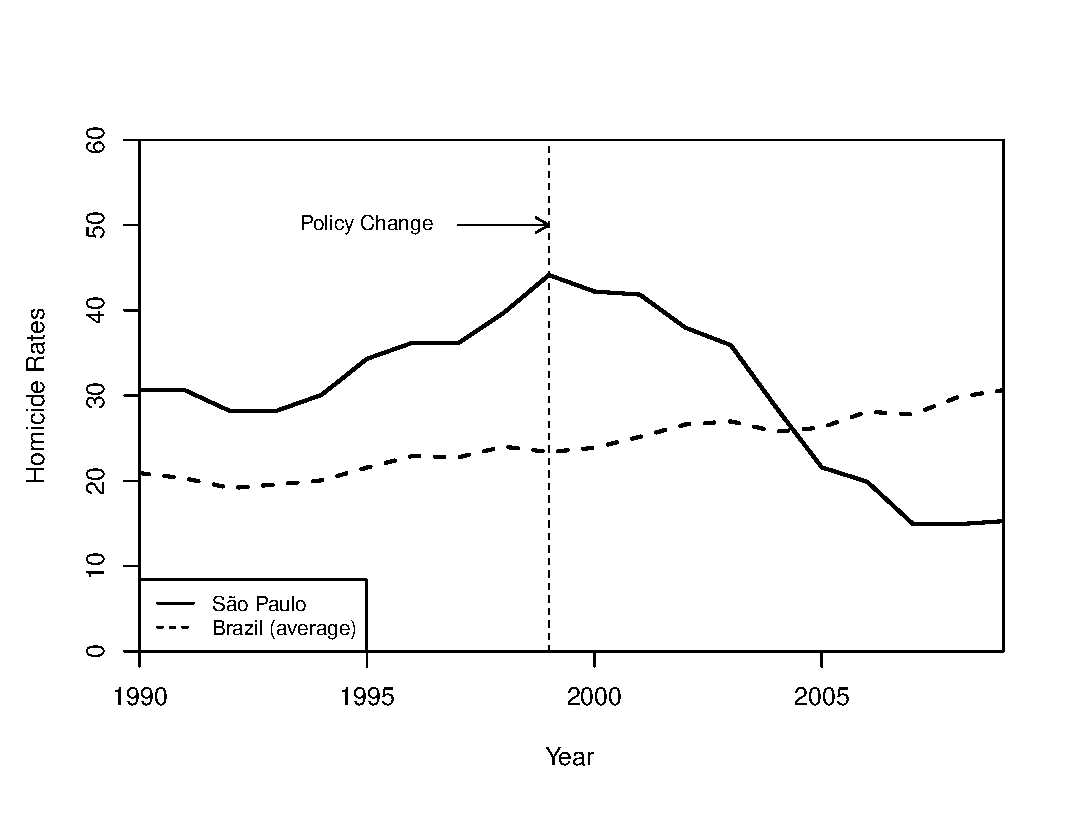
\includegraphics[height=7.5cm]{images/br.eps}
    \caption{Homicide Rates per 100,000 Population -- São Paulo and Brazil (Excluding São Paulo)}
    \label{fig:figure1}
\end{figure}

The trends are even more striking if we consider that deterrence policies are still controversial in the literature. \citet{barbarino2014incapacitation}, \citet{buonanno2013incarceration}, \citet{levitt1996effect,levitt2004understanding} and \citet{owens2009more} claim that incapacitation measures effectively reduce crime, but \citet{eck2006have} and \citet{beattie2007police} suggest that increases in police forces and incarceration rates in the United States and in Canada did not lead to expected outcomes. 

There is good evidence that incapacitation measures have worked well in São Paulo during the last decade. Gun-related homicides have declined about 74\% from 2001 to 2008 \citep{peres2011queda} at the same time when São Paulo has experienced an increase of 770\% in the arrests of repeated murderers \citep[36]{manso2012homicidos}. Although there are studies that indicate possible `hardening effects' of imprisonment, that is, longer sentences may positively affect an individual's tendency to commit further crimes \citep[e.g.][]{chen2007harsher,glaeser1996crime,western2001labor}, the São Paulo case appears to suggest otherwise. Moreover, violent deaths have decreased in all population strata, but especially amongst males (-74.5\%), 15 to 24 year-old men (-78,0\%) and those who live in extreme poverty (-79,3\%), groups that are generally associated with criminality \citep{peres2011queda}.

Nevertheless, it is difficult to know which of the policies have contributed more to this large homicide reduction. Not only we do not have disaggregated data to test preliminary hypotheses, but there may be large interaction effects amongst different public security measures. Therefore, at the moment it is not possible to disentangle micro-level causes from macro effects. But the aggregated impact of the anti-crime policies can be correctly identified if there is no other variable in the causal path leading from the policies mentioned above to our dependent variable (state homicide rates). I argue below that this type of estimation is feasible for the São Paulo case. To back this claim, I suggest that a competing explanation for the homicide drop in São Paulo -- the rise of the PCC -- interferes only with the direct effect of the policies on crime, but not with their \emph{total} effect. In this sense, the synthetic control method provides a plausible identification strategy for my question of interest.

\subsection{Alternative Explanation: The Emergence of the PCC}
\label{sub:alternative_explanation_the_emergence_of_the_pcc}

A recent hypothesis attributes the decrease in violent deaths in São Paulo to the \emph{Primeiro Comando da Capital} (First Command of the Capital, henceforth PCC) \citep{biondi2010, dias2009, dias2011pulverizaccao, de2010crime, de2012governo, willis2015killing}. The PCC is a prison gang that emerged in the early 1990s as a response to the demands of a growing prison population. The PCC provides personal security and financial assistance to their members and affiliates. The gang's internal statute clearly declares that ``[\dots] those who are in liberty [must contribute] to the brothers inside prisons [PCC members] through lawyers, money, help to family members and prison outbreak operations'' \citep{folha2001estatutopcc}.

A group of scholars argue that the PCC significantly contributed to the reduction in violence mainly through the São Paulo prison system. At least since the mid-2000s, these authors argue that the PCC has been able to emerge as an undisputed mediator and solve conflicts between inmates. \citet[83]{dias2009ocupando} writes that ``[\dots] when unable to constitute a universal source of regulation, the official law leaves gaps which are filled by informal instances -- such as the Primeiro Comando da Capital (PCC), in the prisons of São Paulo.'' The gang has implemented informal courts that resemble state institutions, and those meetings have progressively replaced other forms of popular justice such as lynchings or the hiring of target killers \citep[3]{feltran2012metodos}. Moreover, the \emph{Comando} has developed a series of assertive ways to terrorise inmates. Since the PCC's threats are credible, the group is able to impose discipline within the São Paulo prison system \citep{biondi2010,dias2009}.

Paradoxically, the PCC might have also helped to reduce crime in São Paulo by collaborating with street-level police. The Brazilian state does not hold a perfect monopoly of force in many areas of the country \citep{arias2009drugs,de2012governo,hughes2004,pinheiro2000}, thus access to local knowledge may prove vital for the success of a given operation. In this regard, the PCC and the state may collude if the situation is beneficial to both, and as such there is an informal--but potentially unstable--``killing consensus'' in the state \citep{willis2014antagonistic, willis2015killing}.

There has been a vigorous debate over whether the PCC has had a significant impact on violence rates. A few authors see the PCC as the sufficient condition behind the homicide rates decline across São Paulo state \citep{biondi2010, dias2009, dias2011pulverizaccao}, whilst others take a more nuanced view of the role of the prison gang \citep[e.g.][]{willis2015killing}. But both groups of scholars affirm that, based on their first-hand experience, the PCC is the key explanatory variable behind the drop in murders in São Paulo.

Recent econometric works, however, do not seem to confirm that argument. Marcelo Nery has found no convincing results in favour of the `PCC hypothesis' using geo-referenced data for São Paulo \citep{bbc2016pcc}. \citet{biderman2015pax} use anonymous calls to a crime hotline as a proxy for PCC presence in São Paulo city favelas. The authors suggest there is some support for the idea that the criminal syndicate reduces lethal violence in areas under its control, but PCC presence corresponds to only a minor drop in violent crime. Although the PCC impact is not negligible, the gang is not a sufficient condition for the homicide decline.

Another counter-argument to the PCC thesis is that homicides also decreased in areas and groups over which the PCC does not exert control. Firstly, descriptive statistics show that the decline in violent deaths started \emph{before} the PCC's expansion period.\footnote{As shown in figure \ref{fig:figure1}, São Paulo's homicide rates started to drop in 1999. The PCC consolidated their power in the prison system only in the mid-2000s \citep{dias2011pulverizaccao}.} Secondly, the drop in crime was evenly distributed throughout the state: urban and rural areas, small and large cities alike experienced fewer murders.\footnote{See: \url{http://www.fenapef.org.br/27764/} (in Portuguese). Access: July 2016.} Finally, as noted above, \citet{peres2011queda} point out that violent death rates decreased in \emph{all} age groups and social classes in the city São Paulo. Hence, cohorts that do not correspond to typical PCC members (such as the elderly or middle-age females) are also less affected by violence. 

It seems that the influence of the PCC on physical violence has been overstated. It is unlikely that the PCC -- which is underfunded for its size\footnote{A Parliamentary Commission of Inquiry has stated that the PCC earns about 16 million Brazilian Reals per month, which amounts to approximately 60 million US dollars per year. See: \url{http://goo.gl/FwhPa3} (in Portuguese). Access: July 2016. Given the size of the organisation and its undisputed position as the leading crime syndicate in São Paulo, the figures are rather small. As a comparison, Mexico's Sinaloa Cartel profits about 3 billion dollars per year, a sum comparable to the annual earnings of Netflix or Facebook. See: \url{http://nyti.ms/1B09qyV}. Access: July 2016.} -- could have achieved such deep penetration into society and lowered the violence levels across all population groups in the whole state. 

Yet, the group's importance cannot be fully dismissed either. Data on PCC-controlled areas are likely to contain measurement errors that may bias the coefficients, thus caution is required before making strong causal claims on this discussion. Despite mounting observational evidence that the PCC may not provide a complete explanation to São Paulo's lower crime rates, the argument could only be comprehensively tested in a counterfactual case in which the PCC is present and the state policies are not.\footnote{I would like to thank an anonymous reviewer for highlighting this point.} Currently-available data do not allow us to evaluate such scenario.

\subsection{Causal Paths, Moderators, and Total Effects}
\label{sub:causal_paths_moderators_and_total_effects}

A methodological issue remains. If we are to estimate the causal effect of the public measures on the crime rates, how should we proceed? I have noted above that the specific impact of micro-level policies cannot be evaluated due to lack of data. Nonetheless, it is theoretically possible to estimate the \emph{total} effect of policies on crime. 

The difference between direct and total effects can be understood as follows. The direct effect captures the sensitivity of a dependent variable $Y$ to changes in $X$ when this relationship is not mediated by any other variables in the model. Holding all factors constant, the direct effect is a causal chain of length one \citep[160]{sobel1987direct} and could be described simply as $X \rightarrow Y$. In turn, the total effect can be defined as $P(Y_{x} = y)$, that is, ``the probability that response variable $Y$ would take on the value $y$ when $X$ is set to $x$ by external intervention'' \citep[1572]{pearl2001direct}. The total effect is the sum of direct and indirect (or mediated) effects. 

In our case, gun control, incarceration, and police intelligence have likely had a direct effect on homicides. Combined, these variables comprise a direct aggregate policy effect. The omission of a variable measuring the impact of the PCC could bias such an effect, but not interfere with the \emph{total policy effect}. This point is worthy of further consideration. The total policy effect would be unbiased under the assumption that the PCC is in fact a \emph{moderator} between the public policies and the homicide rates, even if the gang's impact over the violence levels is not particularly large. 

Although this argument has rarely been posited in such terms, this position is largely supported by the qualitative literature on the PCC. Fieldwork research generally traces the group's origins and growth to the rising incarceration rates in São Paulo and the need for protection amongst prisoners \citep{dias2011pulverizaccao, manso2014}. Like other prison groups, the PCC would only mobilise resources to provide welfare and act as an arbitrator under the condition that the certainty of punishment by the state is high \citep{skarbek2011, freire2014}. Had the state not increased the costs associated with crime, the prison gang would not have expanded their reach, or even been created in the first place. Hence, the impact of the PCC on street-level violent deaths -- if it exists -- can be safely assumed to be a moderator effect. 

Whereas it would be interesting for researchers to separate these types of effects and isolate the PCC from the other causal outcomes, such estimation is not possible at the state level. However, as these measures were implemented throughout São Paulo state at roughly the same time, their combined effect is computable even though their individual direct effects are not. To do so, it is only necessary to contrast the treated unit (São Paulo) with a counterfactual without the time-assigned treatment (1999 onwards) and evaluate the aggregated effect of the public policies.

This analysis can be estimated in a consistent manner with the synthetic control method. In the following sections I describe how the method creates a valid counterfactual case under a certain set of assumptions. The assumptions are: 1) the PCC is an outcome, not a cause, of the crime-targeting policies; 2) the model does not include unnecessary control variables; 3) interpolation bias is not very severe because the cases in the `donor pool' are relatively similar to the treated unit. 

\section{Methods}
\label{sec:methods}

The synthetic control approach provides an adequate solution for two enduring problems in the social sciences: the arbitrary selection of comparative cases and the poor estimation of causal effects when few pre-treatment observations are available \citep{abadie2003, abadie2010}. With respect to the first issue, scholars often resort to ambiguous criteria in their choice of control units. This practice ends up casting doubts over the validity of their selected counterfactual \citep{abadie2011}. The synthetic method provides a reliable comparative case by adopting a purely data-driven process in order to select a counterfactual. Also, the researcher can still specify what control cases enter the `donor pool.' In this sense, qualitative expert knowledge can be incorporated in the estimation via the selection of cases. 

Regarding the second issue, the accurate estimation of coefficients from a small number of cases, SCM employs a consistent statistical solution to problems of incorrect data extrapolation and model dependence. SCM can be understood as a combination of matching with differences-in-differences. SCM uses matching as a flexible pre-processing tool to reduce imbalance between treated and control units \citep{ho2007matching, rubin1973matching, rubin2006matched}. But unlike matching, SCM deals with only one treated unit over time. Therefore, the method can also be interpreted as a semi-parametric extension to differences-in-differences estimators in which both treated and control units are not required to follow parallel trends in the whole period. \citep{abadie2005semiparametric}. By combining semi-parametric matching with differences-in-differences, SCM provides a rigorous yet versatile method to evaluate time-dependent treatment effects. 

The method works as follows.\footnote{Please refer to Appendix~\ref{sec:synth-appendix} for a formal presentation of the synthetic control method.} SCM starts with the assumption that one case in the sample has received a treatment. The treatment is defined as a time-delimited event that affects the unit of interest, such as the implementation of a new policy or the outbreak of a conflict. SCM also requires a series of control cases to estimate the models, that is, units that did not receive the treatment during the same period. These cases are often related to the treatment case in some meaningful way, and natural choices for the donor pool are provinces within the same country, or states that share important characteristics. These traits can also be more specifically defined and included as quantitative variables in the estimation models. 

SCM then selects a few cases from the donor pool to create a new, artificial control for the treated unit of interest. The main goal of SCM is to construct a counterfactual that resembles the treatment unit more closely than any individual control in the donor pool. Cases are combined in way similar to a weighted average, in which controls that are more similar to the treated unit receive more weights. The weights make explicit the contribution of each separate case to the synthetic control, what also increases the transparency and reliability of the method \citep{abadie2014}. The closer the synthetic control matches the original treated unit before the assignment of the period, the better the quality of the counterfactual. 

The method uses an algorithm to minimise the difference between the control cases and the treated unit before the intervention. The authors adopt the mean squared prediction error (MSPE) as a measure of fit \citep{abadie2003}. MSPE is simply the difference between the fitted and the observed trends of the treatment case. A small value means that the two lines are highly correlated and the artificial control is a good approximation of the missing counterfactual in the post-intervention period. In our case, the counterfactual would be São Paulo from 1999 to 2010 without the crime-reducing policies.

SCM has an intuitive interpretation. Although numeric summaries and other statistics can be obtained from the model, a simple time series graph is usually enough to assess the results. The causal effect is the difference between the treated and the synthetic cohort. The larger the post-treatment gap, the stronger the treatment impact. 

As with all types of observational studies, SCM can also suffer from omitted variable bias. One can never be sure whether all required confounders have been included in a given model. However, the graphical output of the SCM helps diagnose the presence of large disparities between treatment and control cases. If the trends follow similar paths during the control period, it provides some indication -- albeit only informally -- that omitted variable biases are not driving the output. This bias can also be mitigated with expert knowledge. Econometric studies show that the inclusion of a large number of covariates and post-treatment variables to correct for omitted variables bias can actually \emph{worsen} the problem \citep{achen1992social, achen2002toward, clarke2005phantom, clarke2009return, pearl2009causality}. This is particularly true for matching methods. Authors have noted that `over-matching' can lead to severe statistical bias \citep{baser2006too, brookhart2006variable, marsh2002removal}. In this regard, the most plausible solution seems to be attention to the trends and sensible selection of control variables. As I discuss below, the covariates included in this paper are some of the most robust quantitative predictors of homicides.

Furthermore, placebo tests can be run to test the robustness of the findings. For instance, researchers can include `in-time placebos,' dates under which the treatment \emph{did not} occur. Results should change only in the period when the treatment starts and not at any other point in time. Moreover, scholars can also add `in-space placebos' to their models. This test consists of adding different members of the donor pools into the models to see if the estimation varies \citep{abadie2014}. Finally, one can also compare the effects of the treatment of interest by creating a distribution of synthetic cohorts, where every unit (treated or not) is matched with a specific synthetic control case. The parameter of interest should still be relevant. I employ all of these tests in this article and the results can be seen in the following sections.

\section{Data}
\label{sec:data}

I build panel data for the variables \emph{Homicide Rate}, \emph{State GDP per Capita}, \emph{State GDP Growth}, \emph{Years of Schooling}, \emph{Gini Index}, \emph{Natural Logarithm of Population} and \emph{Population Living in Extreme Poverty}. These variables are very common in the specialised literature\footnote{For overviews of cross-national studies of homicide, see \citet{lafree1999summary}, \citet{nivette2011cross} and \citet{trent2012review}.} and represent important social and economic factors I wish to control for. 

The unit of analysis is State-Year. I have data from all of the 26 states plus the capital city (Distrito Federal), ranging from 1990 to 2009. The data for years prior to 1990 are scarce and for years after 2009 have not yet been published. All data used in this paper come from the same source, the \emph{Instituto de Pesquisa Econômica e Aplicada} (IPEA), a government-led research group.\footnote{The data are publicly available at \url{http://www.ipeadata.gov.br/}. The original data files have also been added to \url{https://github.com/danilofreire/homicides-sp-synth} for reproducibility purposes.}

My dependent variable measures the number of homicides per 100,000 inhabitants, which is the most commonly used unit of analysis for lethal violence. This variable was coded by the Brazilian Health Ministry from obituary records, therefore it is less likely than police files to suffer from intentional misrepresentation. 

There are six control variables in the models. \emph{State GDP per Capita} is adjusted in 2010 Brazilian Reals (at the time 1 Brazilian Real bought roughly 0.5 U.S. dollars). \emph{State GDP Growth} is measured in constant 2010 Brazilian Reals and varies by percentage points. \emph{Years of Schooling} describes the average number of years of formal instruction at educational facilities (males and females, 25 years old or more.) \emph{Gini Index} is a measure of inequality, ranging from 0 to 1 where 0 is the most equal and 1 the most unequal. \emph{Natural Logarithm of Population} represents yearly projections of the state population. Since Brazil only runs a census every 10 years, these projections represent the most accurate data available. I have taken the natural logarithm of this variable to account for size effects. Finally, \emph{Population Living in Extreme Poverty} describes the percentage of the state population which do not meet the minimum intake of 2,000 calories per day. This is the only variable that I created specifically for this study. It was coded by simply taking the number of individuals classified as extremely poor by the IPEA and dividing this number by the state's total population.\footnote{\emph{Years of Schooling} and \emph{Gini Index} had a small number of missing observations (about 15 percent) and those cases were imputed with linear interpolation. Both original and imputed variables are available online. See the supplementary appendix for further details on how to replicate this study.} 

\section{Analysis}
\label{sec:analysis}

\subsection{Main Model}

I construct the synthetic cohort (\emph{Synthetic São Paulo}) by imputing information from all of the Brazilian states plus the Federal District. The synthetic control method outputs a set of weights for states and variables such that the treatment state is approximated optimally by these weighted components. This method not only provides a quantitative way of selecting comparison cases but also gives us a much better baseline to compare with the treatment unit. Synthetic São Paulo is constructed using six states, \emph{i.e.}, the six out of the 27 possible cases that received non-zero weights. Table 1 shows that the states that best synthesize São Paulo are, respectively, Santa Catarina (0.274), Distrito Federal (Brasília) (0.210), Espírito Santo (0.209), Rio de Janeiro (0.169), Roraima (0.137) and Pernambuco, which only accounts for 0.01 of the weights. In this regard the state selection does not appear as a complete surprise. Apart from Roraima, the other members of the federation are richer, more densely populated and better schooled than the country average, thus being indeed similar to São Paulo.

\begin{table*}[htp!]
\caption{Synthetic Weights for São Paulo}
\begin{tabular*}{\hsize}
{@{\extracolsep{\fill}}lccc}
\hline
\multicolumn1c{\emph{State}}&\multicolumn1c{\emph{Synthetic Control Weights}}&
\multicolumn1c{\emph{Predictor}}&\multicolumn1c{\emph{Weights}}
\cr
\hline
\emph{Santa Catarina}&0.274
&\emph{Years of Schooling}&0.469
\cr
\emph{Distrito Federal}&0.210
&\emph{State GDP per Capita}&0.275
\cr
\emph{Esp\'{i}rito Santo}&0.209
&\emph{Homicide Rate}&0.241
 \cr
\emph{Rio de Janeiro}&0.169
&\emph{Population Living in Extreme Poverty}&0.009
 \cr
\emph{Roraima}&0.137
&\emph{Gini Index}&0.005
 \cr
 \emph{Pernambuco}&0.001
&\emph{Ln Population}&0.001
 \cr
\hline
\end{tabular*}
\end{table*}
\label{table1}

Among the independent variables, only three out of six receive substantial weights. Given the data I could obtain, the predictors that receive more weight are Years of Schooling (0.469), State GDP per Capita (0.275) and past Homicide Rate (0.241). The three remaining variables are much less relevant to the model. They are, respectively, the Population Living in Extreme Poverty (0.009), Gini Index (0.005) and Natural Logarithm of the Population (0.001). Table 2 compares characteristics of São Paulo and its synthetic control prior to policy implementation. We see that Synthetic São Paulo has very similar coefficients to those of the treatment unit. Moreover, the synthetic control clearly outperforms the sample means in all of the three relevant predictors. The worst measure is State GDP Growth, whose mean is about 2.6 whereas the figure for São Paulo is roughly 1.3 during that period. However, this outcome does not affect the results since the variables that received zero weight were discarded from the models.

\begin{table*}[htp!]
\caption{Homicide Rate Predictor Means Before Policy Implementation}
\begin{tabular*}{\hsize}
{@{\extracolsep{\fill}}lccc}
\hline
\multicolumn1c{\emph{Predictor}}&\multicolumn1c{\emph{São Paulo}}&
\multicolumn1c{\emph{Synthetic São Paulo}}&
\multicolumn1c{\emph{Sample Mean}}
\cr
\hline
\emph{Years of Schooling} & 6.089 & 6.110 & 4.963
\cr
\emph{State GDP Per Capita} & 23.285 & 23.079 & 11.830
\cr
\emph{Homicide Rate} & 32.672 & 32.479 & 21.843
 \cr
\emph{Population Living in Extreme Poverty} & 0.054 & 0.082 & 0.185
 \cr
\emph{Gini Index} & 0.536 & 0.561 & 0.578
 \cr
\emph{Ln Population} & 17.335 & 14.838 & 14.867
\cr
\emph{State GDP Growth} & 1.330 & 2.585 & 3.528
\cr
\hline
\end{tabular*}
\end{table*}
\label{table2}

The results show that the synthetic control method has successfully created a valid counterfactual to our case of interest. Figure \ref{fig:figure2} depicts the evolution of the dependent variable for the treatment and synthetic control cases. We can see that São Paulo and synthetic São Paulo have very close homicide rates series for the period ranging from 1990 until 1998. From 1999 onwards we observe the trajectories departing sharply from each other. The increase in homicide rates shown in the graph is consistent with previous statistical evidence. It indeed confirms that São Paulo had higher than expected levels of lethal violence, which I noted in the first part of this text.

\begin{figure}[H]
    \centering
    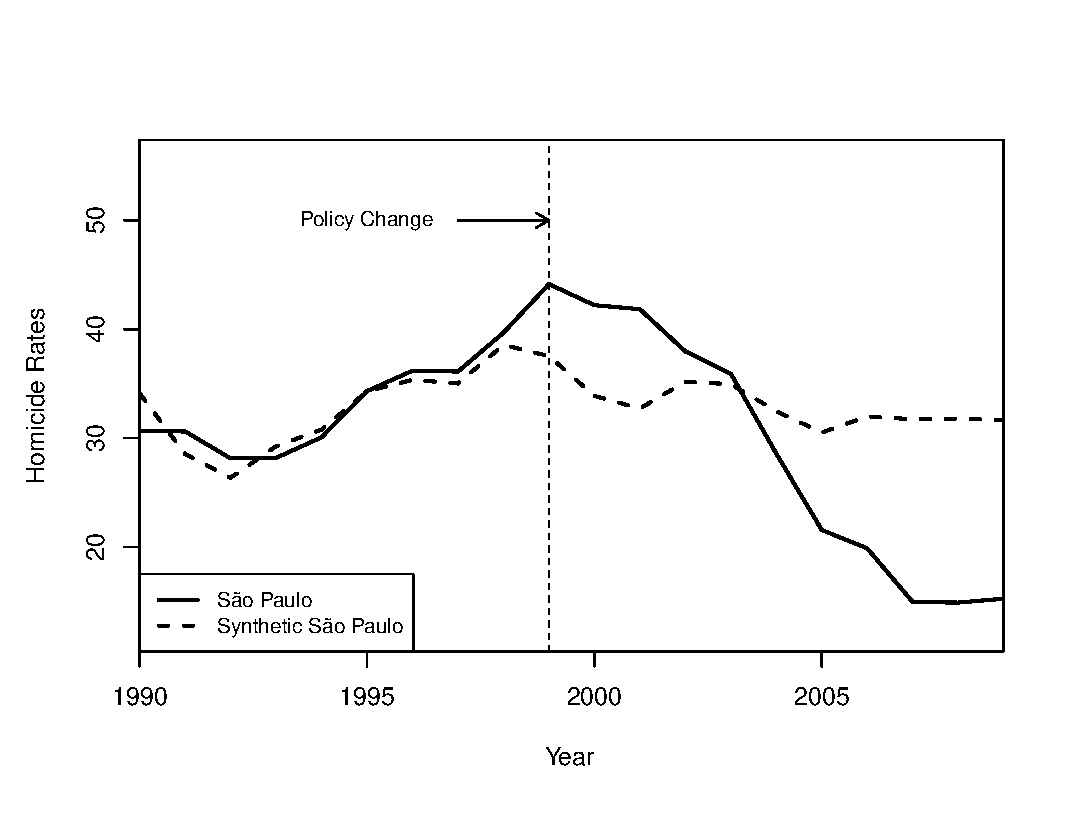
\includegraphics[height=7.5cm]{images/trends.eps}
    \caption{Trends in Homicide Rates: São Paulo versus Synthetic São Paulo}
    \label{fig:figure2}
\end{figure}

Despite the high levels of violence in 1999 -- when the new crime-reducing programme was implemented -- the number of homicides consistently declined until 2009. The trend is indeed monotonic and there is not a single peak in homicide rates after the policies have been put into practice. I interpret that as strong evidence in favour of the public policies. 

\begin{figure}[H]
    \centering
    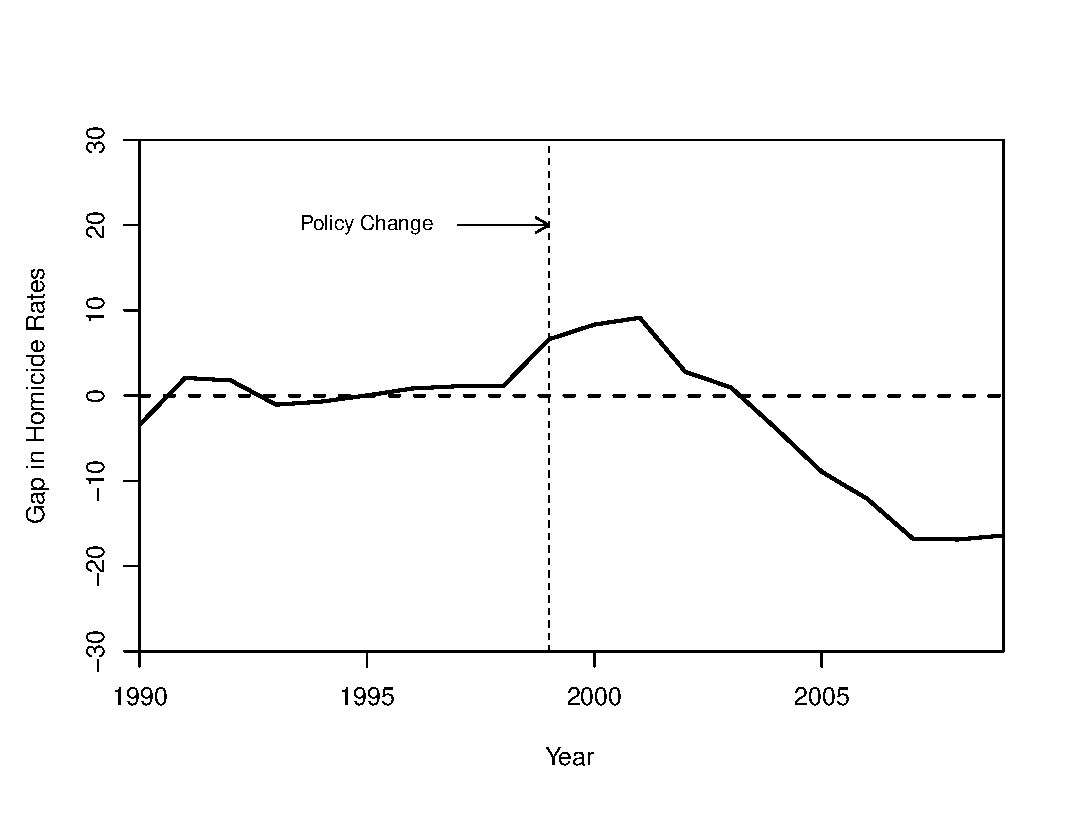
\includegraphics[height=7.5cm]{images/gaps.eps}
    \caption{Homicide Rates Gap between São Paulo and Synthetic São Paulo}
    \label{fig:figure3}
\end{figure}

With respect to the size of the effect, in 1998 the homicide rate in São Paulo was around 40 deaths per 100,000 inhabitants. In 2009 -- the last year for which data are available -- the rate dropped to 15, whereas synthetic São Paulo observed above 30 deaths per 100,000. That means a gap of $-20$ deaths for every 100,000 people in São Paulo in 2009, as can be seen in Figure \ref{fig:figure3}. I estimate that the new policies implemented in São Paulo saved roughly 20,300 lives in the period from 1999 to 2009.\footnote{My estimate of lives saved by the policies implemented in São Paulo is done as follows. I consider the years after policy implementation (1999--2009), then I sum the number of homicides in São Paulo in that period. This gives us 124,077 homicides between 1999 and 2009. I do the same procedure for the synthetic São Paulo; I sum the number of homicides in each state that makes the synthetic control in the period, while adjusting the contribution of each of these states by their respective weights in the synthesis. The number of homicides in synthetic São Paulo between 1999 and 2009 is 144,408. Finally, I subtract the number of homicides in the control by the number of homicides in the treatment. The result is 20,331 lives saved.} It is important to mention that the homicide rate in São Paulo continues to drop by the year, while the same is not happening in the rest of the country. 

\subsection{Robustness Checks}

To further analyse the findings, I run five robustness tests. I first create an `in-time placebo' synthetic control. This test consists of creating a false starting date for the intervention period to check if one could observe false treatment effects in the pre-treatment years \citep{abadie2014}. If that were to be the case, the validity of the main results could be put into question. The result of this placebo test can be seen in Figure \ref{fig:figure4}. When I run the model with 1994 as the year when there was a supposed policy change, the result shows that there is only a minor gap between both lines. In other words, the method does not indicate a definite departure of trends between treatment and control cases. 

\begin{figure}[H]
    \centering
    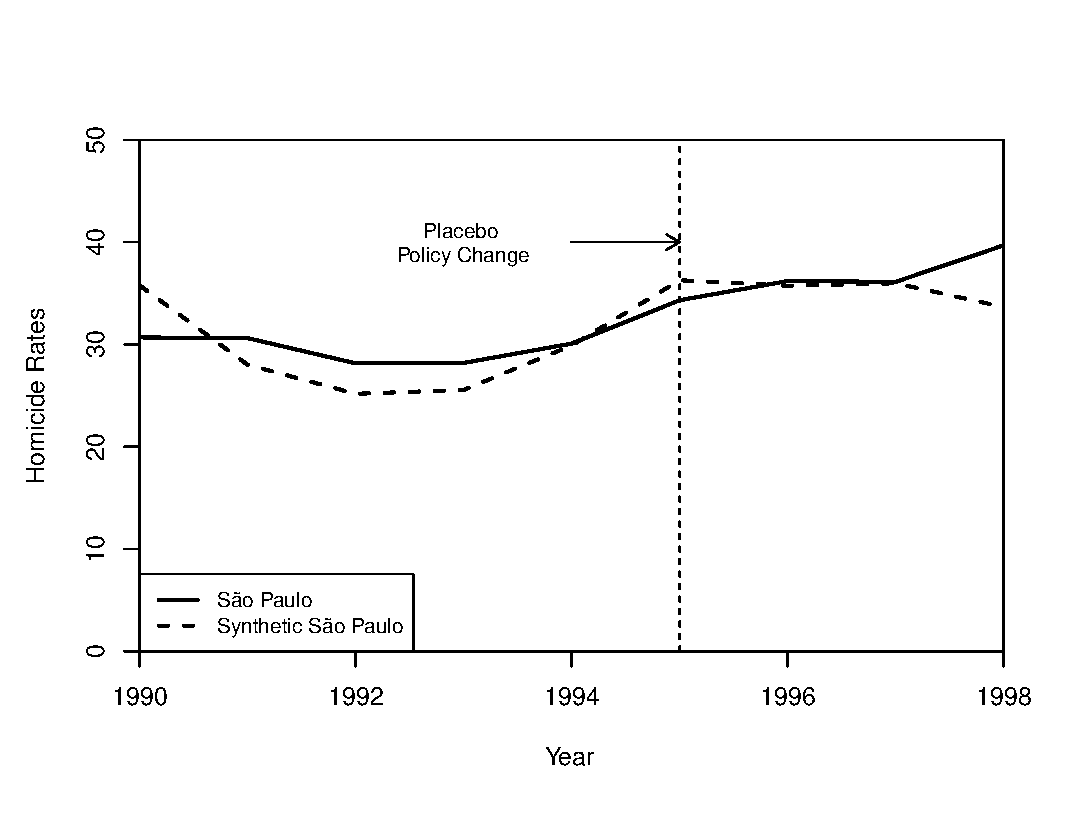
\includegraphics[height=7.5cm]{images/placebo.eps}
    \caption{Placebo Policy Implementation in 1994: São Paulo versus Synthetic São Paulo}
    \label{fig:figure4}
\end{figure}

I also conducted a leave-one-out robustness test. In this test I drop the states composing the synthetic control one at a time. The main goal of this analysis is to evaluate whether a single control state is driving the results. This would suggest that the original synthetic control -- which is composed of five states at a time -- is probably not a reasonable counterfactual. The results of this analysis can be found in Figure \ref{fig:figure5}. We see that the synthetic control (dashed line) is a reasonable amalgam of cases. Also, because the relative positions of treatment and controls are stable across controls, we observe that no control state is biasing the estimates.

\begin{figure}[H]
    \centering
    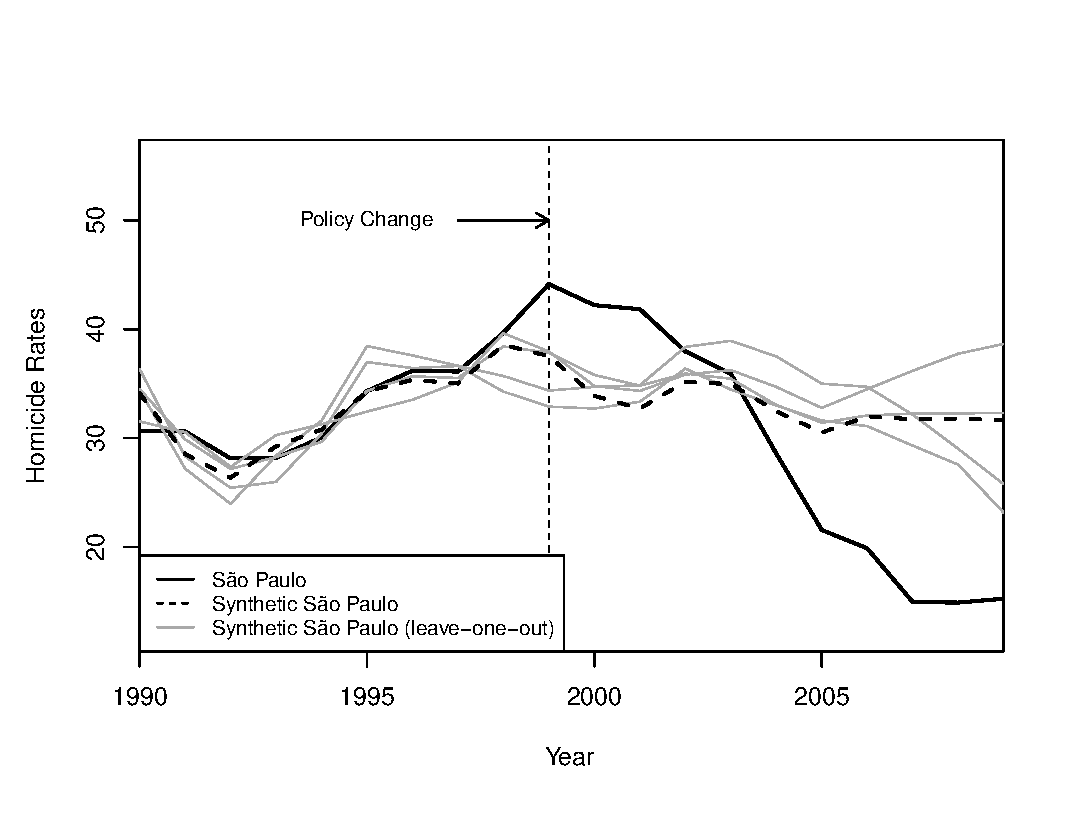
\includegraphics[height=7.5cm]{images/leave-one-out.eps}
    \caption{Leave-One-Out Distribution of the synthetic Control for São Paulo}
    \label{fig:figure5}
\end{figure}

Figure \ref{fig:figure6} shows the difference in homicide rates between the treated units and their synthetic controls. Here I estimate a synthetic control case for São Paulo and for each of the other 26 Brazilian states. This test assesses whether there is any previously unobserved national or regional trend that explains the original results. We observe that in São Paulo the homicide rate gap increases consistently during the treatment period, whereas the lines for the other states are moving randomly. Several lines fail to show any substantial difference between the state line and that of its synthetic counterfactual case. This indicates the results for São Paulo are unlikely to be a result of broader trends.

\begin{figure}[H]
    \centering
    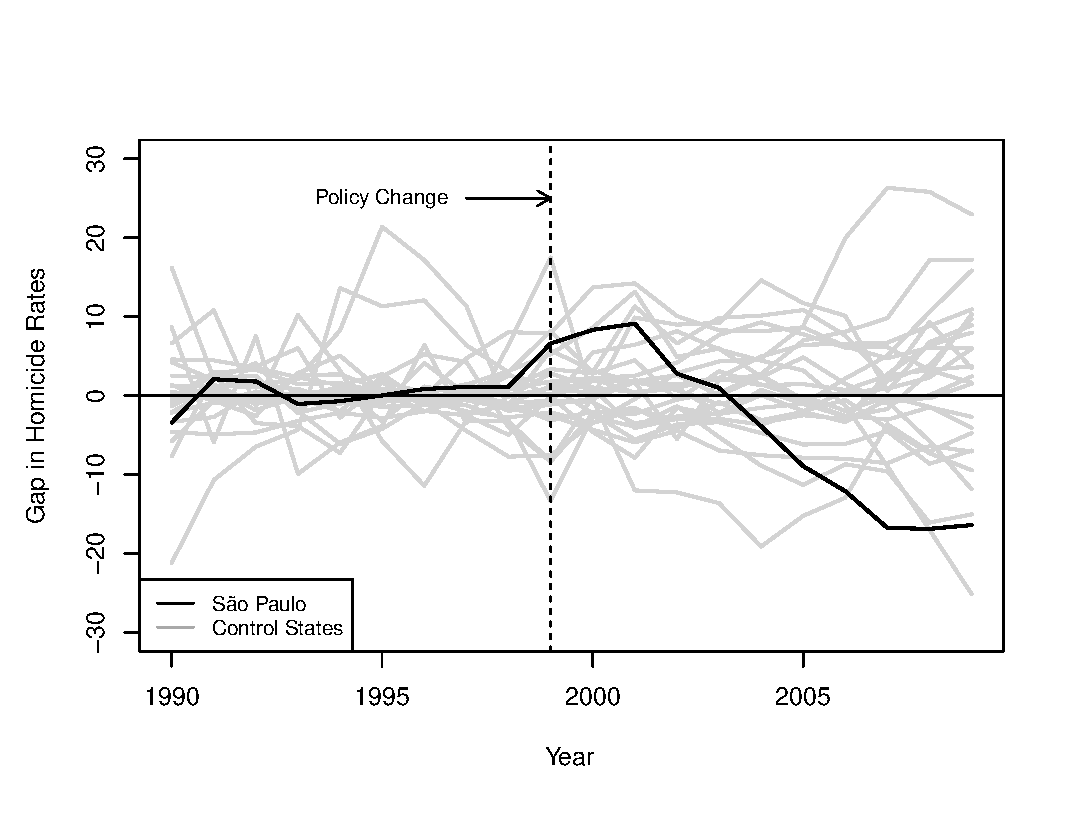
\includegraphics[height=7.5cm]{images/permutation-gaps2.eps}
    \caption{Permutation Test: Homicide Rate Gaps in São Paulo and 26 Control States}
    \label{fig:figure6}
\end{figure}

Figure \ref{fig:figure7} presents the same test displayed in figure \ref{fig:figure6}, but it uses a stricter threshold for the simulated synthetic controls. The graph features cases in which the mean squared prediction error, a measure of goodness-of-fit, is no higher than twice that of São Paulo. That is, only placebos that have good synthetic matches were selected for the analysis \citep[503]{abadie2010}.  In this group, the negative gap for the homicide rate São Paulo is by far the most relevant, providing further evidence for the original findings.

\begin{figure}[H]
    \centering
    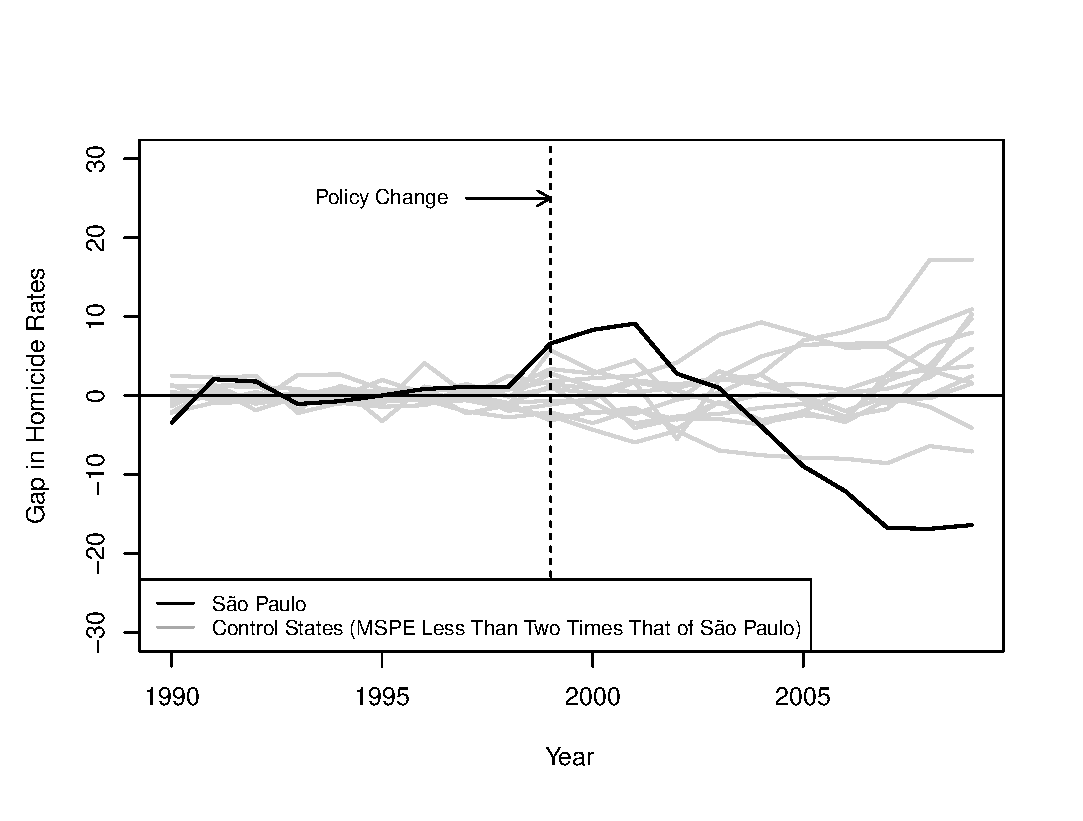
\includegraphics[height=7.5cm]{images/low-mspe.eps}
    \caption{Permutation Test: Homicide Rate Gaps in São Paulo and Selected Control States}
    \label{fig:figure7}
\end{figure}

Lastly, I estimate another synthetic control using another approach. Here, I employ a Bayesian structural time-series model to verify the stability of the previous results \citep{brodersen2015inferring}. This inference procedure is similar to that described in section \ref{sec:methods} and it also consists of matching pre-treatment values of the unit of interest, São Paulo, to other potential control states. However, in this model only the time trends of the dependent variable are matched. In a sense, this is closer to a traditional differences-in-differences approach, but without the restrictive assumption that the treated and the control cases would follow parallel trends over time \citep[494]{abadie2010}.  

\begin{figure}[H]
    \centering
    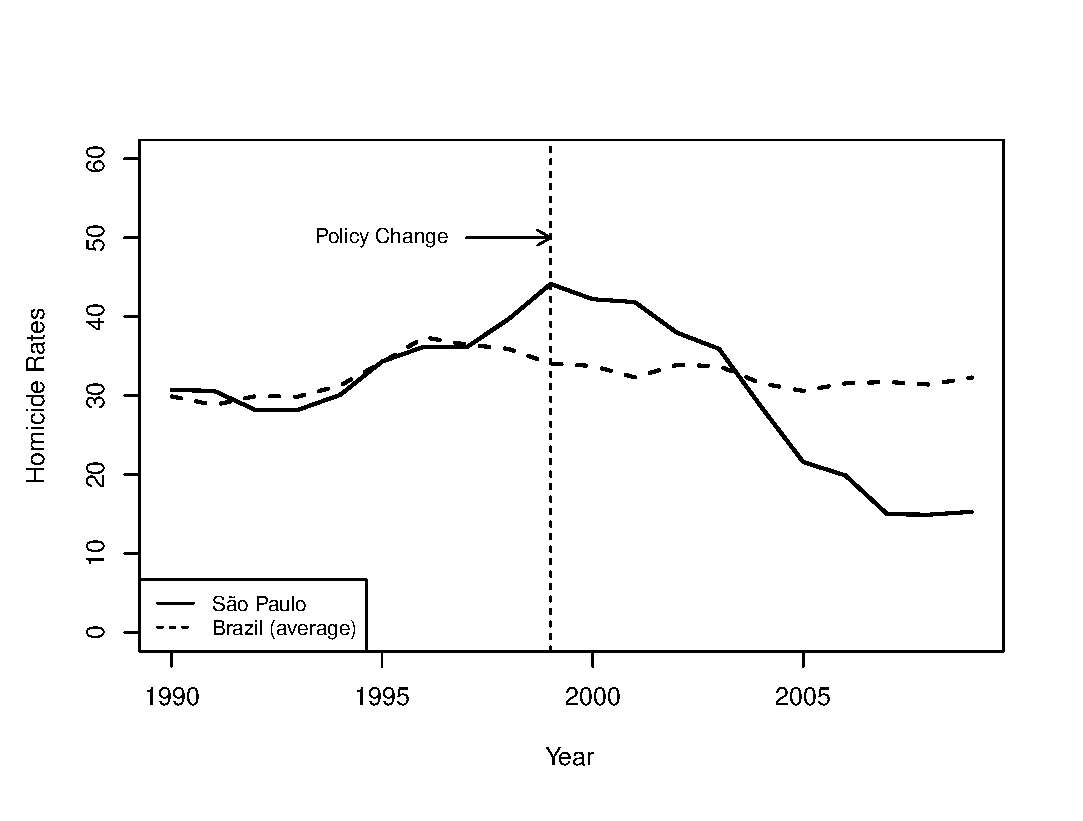
\includegraphics[height=7.5cm]{images/causal-impact.eps}
    \caption{Bayesian Structural Time Series Model: São Paulo and Synthetic São Paulo}
    \label{fig:figure8}
\end{figure}

The model shows that in 2009 we should have expected São Paulo to have a homicide rate equal to 32.3 deaths per 100,000, but we observe only 15.2. Thus, the actual rate in São Paulo corresponds to only 47\% of the expected counterfactual. The method also generates an estimate for the probability of causal effect. The calculations indicate a 96.3\% chance of a causal impact in the period. In this sense, it is unlikely that the results are a statistical fluke.

\section{Conclusion}
\label{sec:conclusion}

As I have hopefully demonstrated, when compared to a synthetic control case, homicide rates were drastically reduced in São Paulo. Although it is not possible to estimate the treatment effect of each specific policy implemented during the 1990s and 2000s, I suggest that their aggregate impact is surely not negligible. If the estimation strategy employed in this paper is correct, the state of São Paulo offers an example that it is feasible to fight crime with targeted policies. This as an encouraging result, as it suggests that governments can make progress in reducing crime with the resources they already have at hand and need not rely exclusively upon structural conditions that are largely beyond their control, such as unemployment, per capita income and inequality. Robustness tests provide further evidence for my findings.

I also argue in favour of the synthetic control method as a tool to evaluate government policies. This approach offers an intuitive way to assess causality claims when there is only a single treated unit and it can be easily applied in a great number of situations. Assuming that there is a reasonable number of potential cases in the `donor pool,' a synthetic control can be meaningfully compared to the actual case. In this way, the technique allows the researcher to use the potential outcomes framework even in unusual conditions.

Future research can extend the present findings in a number of ways. First, it would be interesting to test whether other criminal activities have been affected by the state government policies I mentioned previously. Since property crimes are pervasive in São Paulo, scholars could evaluate the causal link (or lack thereof) between public policies and the incidence of theft or robberies. Unfortunately, several states in Brazil do not publish time-series data for property crime, so I could not use the synthetic control method for that dependent variable. As more data become available, this will create an interesting opportunity for investigation. Secondly, micro-level studies are needed to clarify the mechanisms behind São Paulo's homicide reduction, and isolate direct from indirect effects of each individual policies. Due to the shortage of data on targeted policies, qualitative research may explain what the motivations, successes and shortcomings of São Paulo's recent security measures were. Finally, there are still unresolved questions with regards to the `PCC hypothesis', and this is a promising avenue for future academic work. New research could provide insights into how public policies work and, hopefully, help public authorities to design more effective policies against crime.

\section{Appendix} 
\label{sec:synth-appendix}

\subsection{The Synthetic Control Estimator}
\label{sec:synth-estimator}

This appendix presents a formal presentation of the synthetic control estimator. Let $j = 1, \dots, J + 1$ be a series of units in periods $t = 1, \dots, T$. In our case, the units are the 27 Brazilian federal states and the time period spans from 1990 to 2009. Assuming that the first unit, São Paulo, has been exposed to the treatment, we have $J$ control units to be included in the case studies donor pool, \emph{i.e.} the 26 remaining states. We define treatment as the series of post-1999 government anti-crime policies implemented in the São Paulo.

Let $Y_{it}^N$ be the homicide rate that would be observed for unit $i$, São Paulo, at time $t$ with no treatment (1990--1998). Conversely, let $Y_{it}^I$ be the observable outcome for unit $i$ at time $t$ had it been subjected to the treatment in periods $T_{0} + 1$ to $T$ (1999--2009). An important assumption is that the treatment has no effect on unit $i$ before the date of intervention, therefore, the values for São Paulo with and without the policy interventions are the same for the pre-treatment period (1990--1998). In formal terms, $Y_{it}^I = Y_{it}^N$ $\forall t < T_{0}$. The observed outcome is defined by $Y_{it}^I = Y_{it}^N + \alpha_{it}D_{it}$, where $\alpha_{it}$ is the effect of crime-reducing policies on homicide rates, and $D_{it}$ is a binary variable that takes the value of $1$ if we refer to post-intervention period (after 1999) and $0$ otherwise. The goal of this paper is to estimate $\alpha_{it}$, the effect of the treatment (homicide reduction policies), for the state of São Paulo for all $t \geq T_0$, that is, from 1999 to 2009. However, we cannot observe São Paulo \emph{without} those policies, as there is no way for the state to have and not have the intervention at the same time. This is what \citet{holland1986} calls the ``fundamental problem of causal inference'': only one of the outcomes of interest is measurable at any given time.

But although we cannot accurately know how São Paulo would be without the treatment, we can approximate it by using a weighted average of the remaining Brazilian states such that $Y_{it}^N = \delta_{t} + \theta_{t}Z_{i} + \lambda_{t}\mu_{i} + \epsilon_{it}$. In this model, $\delta_{t}$ is an unobserved time-dependent factor common to all cases, $Z_{i}$ is a $(1 \times r)$ vector of observed control variables not affected by the policy, $\theta_{t}$ is a $(r \times 1)$ vector of unknown time-specific parameters, $\lambda_{t}$ is a $(1 \times F)$ vector of unknown common factors to all states, $\mu_{i}$ is a state-specific unobservable variable and $\epsilon_{it}$ represents unobserved transitory shocks with mean $0$ for all units (error term). Basically, what SCM tries to do is to match $Z_{i}$, the control variables, and the pre-treatment $Y_{it}$ of São Paulo (1990--1998) so that $\mu_{i}$ is matched as a result.

Synthetic São Paulo is the weighted average of the other 26 Brazilian states. Thus, it is a $(J \times 1)$ vector of weights $W = (w_2 , \dots, w_{J+1})'$ with $w_j \geq 0$ for $j = 2, \dots, J + 1$ and $w_2 + \dots + w_{J+1} = 1$. Each of the elements included in $W$ represents a specific weighted average of control states, that is, a potential synthetic control for São Paulo. The idea is to select a case that resembles São Paulo as closely as possible. Let $X_{1}$ be a $(k \times 1)$ vector of pre-1999 predictor variables for São Paulo and let $X_{0}$ be a $(k \times J)$ matrix containing the predictor variables for the potential control states. Let $\bar{Y}_{i}^{K_{1}}, \dots, \bar{Y}_{i}^{K_{M}}$ be $M$ linear functions of pre-treatment outcomes $(M \geq F)$. One can choose $w^*$ such that:

$$\sum_{j = 2}^{J + 1} w_{j}^{*} Z_{j} = Z_{1}, \sum_{j = 2}^{J + 1} w_{j}^{*}\bar{Y}_{j}^{K_{1}} = \bar{Y}_{1}^{K_{1}}, \dots, \sum_{j = 2}^{J + 1} w_{j}^{*}\bar{Y}_{j}^{K_{M}} = \bar{Y}_{1}^{K_{M}}$$ 

Consequently, as noted by Abadie and his collaborators (\citeyear{abadie2010}), if $T_{0}$ is sufficiently large when compared to the scale of $\epsilon_{it}$, an approximately unbiased estimator for $\alpha_{1t}$, the effect of public security policies in São Paulo, can be described by:

$$\hat{\alpha}_{1t} = Y_{1t} - \sum_{j = 2}^{J + 1} w_{j}^{*} Y_{jt}$$

for all $t \in \left\{T_{0} + 1, \dots, T \right\}$, that is, after the intervention period (1999--2009). In practice, $W^{*}$ is chosen non-parametrically as to minimise $||X_{1} - X_{0}W||$, subject to the weight constrains. Consider $||X_{1} - X_{0}W||v = \sqrt{(X_{1} - X_{0}W)'V (X_{1} - X_{0}W)}$, where $V$ is a $(k \times k)$ symmetric and semi-definite positive matrix with the relative importance of each assigned homicide rate predictor. From various possible ways of choosing $V$, here I follow the recommendation of \citet{abadie2003} and choose $V^{*}$ as the value of $V$ that minimises the root mean squared prediction error (RMSPE) for homicide rates in the entire pre-treatment period (1990-1998).


\subsection{\texttt{R} Code}
\label{sec:synth-code}

The \texttt{R} code below replicates all statistical analyses and graphs included in this chapter. The original data files as well as the final dataset are available at \href{https://github.com/danilofreire/homicides-sp-synth}{https://github.com/danilofreire/homicides-sp-synth}. 

\singlespacing
\small
\begin{verbatim}
######################
### Data Wrangling ###
######################

# Please set your working directory to the data/ folder

# Clear the workspace
rm(list = ls())

# Load necessary packages
library(reshape2)  # data manipulation

# Dependent variable:
dep <- read.csv("homicide-rates.csv", header = TRUE, skip = 1)

dep.molten <- melt(dep,
                   id.vars = c("Sigla",
                               "Código",
                               "Estado")
                    )

colnames(dep.molten) <- c("abbreviation",
                          "code",
                          "state",
                          "year",
                          "homicide.rates")

dep.molten$year <- as.numeric(substring(dep.molten$year, 2))
\end{verbatim}

\newpage

\begin{verbatim}
# Independent variables
ind1 <- read.csv("state-gdp-capita.csv", header = TRUE, skip = 1)

ind1.molten <- melt(ind1,
                    id.vars = c("Sigla",
                                "Código",
                                "Estado")
                    )

colnames(ind1.molten) <- c("abbreviation",
                           "code",
                           "state",
                           "year",
                           "state.gdp.capita")

ind1.molten$year <- as.numeric(substring(ind1.molten$year, 2))

ind2 <- read.csv("state-gdp-growth-percentage.csv", header = TRUE, skip = 1)

ind2.molten <- melt(ind2,
                    id.vars = c("Sigla",
                                "Código",
                                "Estado")
                    )

colnames(ind2.molten) <- c("abbreviation",
                           "code",
                           "state",
                           "year",
                           "state.gdp.growth.percent")

ind2.molten$year <- as.numeric(substring(ind2.molten$year, 2))

ind3 <- read.csv("gini.csv", header = TRUE, skip = 1)

ind3.molten <- melt(ind3,
                    id.vars = c("Sigla",
                                "Código",
                                "Estado")
                    )

colnames(ind3.molten) <- c("abbreviation",
                           "code",
                           "state",
                           "year",
                           "gini")

ind3.molten$year <- as.numeric(substring(ind3.molten$year, 2))

ind4 <- read.csv("population-projection.csv",
                 header = TRUE,
                 skip   = 1)

ind4.molten <- melt(ind4,
                    id.vars = c("Sigla",
                                "Código",
                                "Estado")
                    )

colnames(ind4.molten) <- c("abbreviation",
                           "code",
                           "state",
                           "year",
                           "population.projection")

ind4.molten$year <- as.numeric(substring(ind4.molten$year, 2))

ind5 <- read.csv("population-extreme-poverty.csv", header = TRUE, skip = 1)

ind5.molten <- melt(ind5,
                    id.vars = c("Sigla",
                                "Código",
                                "Estado")
                    )

colnames(ind5.molten) <- c("abbreviation",
                           "code",
                           "state",
                           "year",
                           "population.extreme.poverty")

ind5.molten$year <- as.numeric(substring(ind5.molten$year, 2))

ind6 <- read.csv("years-schooling.csv", header = TRUE, skip = 1)

ind6.molten <- melt(ind6,
                    id.vars = c("Sigla",
                                "Código",
                                "Estado")
                    )

colnames(ind6.molten) <- c("abbreviation",
                           "code",
                           "state",
                           "year",
                           "years.schooling")

ind6.molten$year <- as.numeric(substring(ind6.molten$year, 2))

# Merges files
data.list <- list(dep.molten,
                  ind1.molten,
                  ind2.molten,
                  ind3.molten,
                  ind4.molten,
                  ind5.molten,
                  ind6.molten)

data1 <- Reduce(function(...) merge(..., all = TRUE), data.list)

# Subset and sort
data2 <- subset(data1, year >= 1990 & year <= 2009)
data2 <- data2[order(data2$state), ]
rownames(data2) <- NULL

# Count missing observations, calculate their percentage
round(sapply(data2, function(x) length(which(is.na(x)))), 2)
round(sapply(data2, function(x) length(which(is.na(x)))/length(x)), 2)

# Linear imputation of missing values.
data2$gini.imp <- approxfun(seq_along(data2$gini), data2$gini)(seq_along(data2$gini))

data2$population.extreme.poverty.imp <- approxfun(seq_along(data2$population.extreme.poverty),
data2$population.extreme.poverty)(seq_along(data2$population.extreme.poverty))

data2$years.schooling.imp <- approxfun(seq_along(data2$years.schooling),
data2$years.schooling)(seq_along(data2$years.schooling))

# Create proportion.extreme.poverty
data2$proportion.extreme.poverty <- data2$population.extreme.poverty.imp / data2$population.projection

# Transform variables to improve interpretation
data2$population.projection.ln <- log(data2$population.projection)

# Save data as df.csv
write.table(data2,
            "df.csv",
            row.names = FALSE,
            col.names = TRUE,
            sep       = ",")
            
#####################
### Data Analysis ###
#####################

# Load necessary packages
library(dplyr) # data manipulation
library(Synth) # models

# Load data
df <- read.csv("df.csv", header = TRUE)

# Prepare dataset
df$state <- as.character(df$state) # required by dataprep()

# Plot: Homicide rates for Sao Paulo and Brazil (average)
df1 <- df %>%
        mutate(homicide.sp = ifelse(homicide.rates & state == "São Paulo", homicide.rates, NA)) %>%
        select(year, homicide.sp)

df2 <- df %>%
        mutate(homicide.rates1 = ifelse(homicide.rates & state != "São Paulo", homicide.rates, NA)) %>%
        group_by(year) %>%
        summarise(homicide.br = mean(homicide.rates1, na.rm = TRUE))

setEPS()
postscript(file    = "br.eps",
           horiz   = FALSE,
           onefile = FALSE,
           width   = 7,     # 17.8 cm
           height  = 5.25)  # 13.3 cm

plot(x = df1$year,
     y = df1$homicide.sp,
     type = "l",
     ylim = c(0, 60),
     xlim = c(1990, 2009),
     xlab = "Year",
     ylab = "Homicide Rates",
     cex = 3,
     lwd = 2,
     xaxs = "i",
     yaxs = "i"
)

lines(df2$year,
      df2$homicide.br,
      lty = 2,
      cex = 3,
      lwd = 2)

arrows(1997, 50, 1999, 50,
       col    = "black",
       length = .1)

text(1995, 50,
     "Policy Change",
     cex = .8)

abline(v   = 1999,
       lty = 2)

legend(x = "bottomleft",
       legend = c("São Paulo",
                  "Brazil (average)"),
       lty    = c("solid", "dashed"),
       cex    = .8,
       bg     = "white",
       lwdc(2, 2)
)

invisible(dev.off())

# Prepare data for synth
dataprep.out <-
        dataprep(df,
                 predictors = c("state.gdp.capita",
                                "state.gdp.growth.percent",
                                "population.projection.ln",
                                "years.schooling.imp"
                                ),
                 special.predictors = list(
                         list("homicide.rates", 1990:1998, "mean"),
                         list("proportion.extreme.poverty", 1990:1998, "mean"),
                         list("gini.imp", 1990:1998, "mean")
                         ),
                 predictors.op = "mean",
                 dependent     = "homicide.rates",
                 unit.variable = "code",
                 time.variable = "year",
                 unit.names.variable   = "state",
                 treatment.identifier  = 35,
                 controls.identifier   = c(11:17, 21:27, 31:33, 41:43, 50:53),
                 time.predictors.prior = c(1990:1998),
                 time.optimize.ssr     = c(1990:1998),
                 time.plot             = c(1990:2009)
                 )

# Run synth
synth.out <- synth(dataprep.out)

# Get result tables
print(synth.tables   <- synth.tab(
        dataprep.res = dataprep.out,
        synth.res    = synth.out)
      )

# Plot: Main model
setEPS()
postscript(file    = "trends.eps",
           horiz   = FALSE,
           onefile = FALSE,
           width   = 7,     # 17.8 cm
           height  = 5.25)  # 13.3 cm

path.plot(synth.res    = synth.out,
          dataprep.res = dataprep.out,
          Ylab         = c("Homicide Rates"),
          Xlab         = c("Year"),
          Legend       = c("São Paulo","Synthetic São Paulo"),
          Legend.position = c("bottomleft")
)

abline(v   = 1999,
       lty = 2)

arrows(1997, 50, 1999, 50,
       col    = "black",
       length = .1)

text(1995, 50,
     "Policy Change",
     cex = .8)

invisible(dev.off())

# Main model: gaps plot
setEPS()
postscript(file    = "gaps.eps",
           horiz   = FALSE,
           onefile = FALSE,
           width   = 7,
           height  = 5.25)

gaps.plot(synth.res    = synth.out,
          dataprep.res = dataprep.out,
          Ylab         = c("Gap in Homicide Rates"),
          Xlab         = c("Year"),
          Ylim         = c(-30, 30),
          Main         = ""
)

abline(v   = 1999,
       lty = 2)

arrows(1997, 20, 1999, 20,
       col    = "black",
       length = .1)

text(1995, 20,
     "Policy Change",
     cex = .8)

invisible(dev.off())

## Calculating how many lives were saved during the treatment period

# Weights below retrieved form dataprep.out
# State Code  State Weight  State Name        State Abbreviation
# 42          0.274         Santa Catarina    SC
# 53          0.210         Distrito Federal  DF
# 32          0.209         Espirito Santo    ES
# 33          0.169         Rio de Janeiro    RJ
# 14          0.137         Roraima           RR
# 14          0.001         Pernambuco        PB
# 35          treat         Sao Paulo         SP
\end{verbatim}

\begin{verbatim}
# Get years after policy change
df.2 <- df[which(df$year >= 1999),]

# Calculate total number of deaths in SP
num.deaths.sp <- sum( (df.2$homicide.rates[which(df.2$abbreviation == "SP")])/100000 *
    (df.2$population.projection[which(df.2$abbreviation == "SP")]))

# Calculate estimated number of deaths in Synthetic São Paulo
num.deaths.synthetic.sp <- sum( (0.274 * (df.2$homicide.rates[which(df.2$abbreviation == "SC")])/100000 *
(df.2$population.projection[which(df.2$abbreviation == "SP")]))
                                + (0.210 * (df.2$homicide.rates[which(df.2$abbreviation == "DF")])/100000 *
                                (df.2$population.projection[which(df.2$abbreviation == "SP")]))
                                + (0.209 * (df.2$homicide.rates[which(df.2$abbreviation == "ES")])/100000 *
                                (df.2$population.projection[which(df.2$abbreviation == "SP")]))
                                + (0.169 * (df.2$homicide.rates[which(df.2$abbreviation == "RJ")])/100000 *
                                (df.2$population.projection[which(df.2$abbreviation == "SP")]))
                                + (0.137 * (df.2$homicide.rates[which(df.2$abbreviation == "RR")])/100000 *
                                (df.2$population.projection[which(df.2$abbreviation == "SP")]))
                                + (0.001 * (df.2$homicide.rates[which(df.2$abbreviation == "PB")])/100000 *
                                (df.2$population.projection[which(df.2$abbreviation == "SP")]))
                                )

lives.saved <- num.deaths.synthetic.sp - num.deaths.sp
lives.saved # Between 1999 and 2009

########################
### Robustness Tests ###
########################

# Prepare dataset
df$state <- as.character(df$state) # required by dataprep()

## Placebo Test -- Control ends in 1994
dataprep.out1 <-
        dataprep(df,
                 predictors = c("state.gdp.capita",
                                "state.gdp.growth.percent",
                                "population.projection.ln",
                                "years.schooling.imp"
                 ),
                 special.predictors = list(
                         list("homicide.rates", 1990:1994, "mean"),
                         list("proportion.extreme.poverty", 1990:1994, "mean"),
                         list("gini.imp", 1990:1994, "mean")
                 ),
                 predictors.op = "mean",
                 dependent     = "homicide.rates",
                 unit.variable = "code",
                 time.variable = "year",
                 unit.names.variable   = "state",
                 treatment.identifier  = 35,
                 controls.identifier   = c(11:17, 21:27, 31:33, 41:43, 50:53),
                 time.predictors.prior = c(1990:1994),
                 time.optimize.ssr     = c(1990:1994),
                 time.plot             = c(1990:1998))

# Run synth
synth.out1 <- synth(dataprep.out1)

# Get result tables
print(synth.tables   <- synth.tab(
        dataprep.res = dataprep.out1,
        synth.res    = synth.out1)
      )

# Placebo test: graph
setEPS()
postscript(file    = "placebo.eps",
           horiz   = FALSE,
           onefile = FALSE,
           width   = 7,
           height  = 5.25)

path.plot(synth.res       = synth.out1,
          dataprep.res    = dataprep.out1,
          Ylab            = c("Homicide Rates"),
          Xlab            = c("Year"),
          Legend          = c("São Paulo","Synthetic São Paulo"),
          Legend.position = c("bottomleft"),
          Ylim            = c(0, 50)
)

abline(v   = 1995,
       lty = 2)

arrows(1994, 40, 1995, 40,
       col    = "black",
       length = .1)

text(1993, 40,
     "Placebo \nPolicy Change",
     cex = .8)

invisible(dev.off())

## Leave-one-out

# Loop over leave one outs
storegaps <- matrix(NA, length(1990:2009), 4)

colnames(storegaps) <- c(14, 33, 42, 53) # RR, RJ, SC, DF
co <- unique(df$code)
co <- co[-25]

for(k in 1:4){

        # Data prep for training model
        omit <- c(14, 33, 42, 53)[k]

        # Prepare data for synth
        dataprep.out2 <-
                dataprep(df,
                         predictors = c("state.gdp.capita",
                                        "state.gdp.growth.percent",
                                        "population.projection.ln",
                                        "years.schooling.imp"
                         ),
                         special.predictors = list(
                                 list("homicide.rates", 1990:1998, "mean"),
                                 list("proportion.extreme.poverty", 1990:1998, "mean"),
                                 list("gini.imp", 1990:1998, "mean")
                         ),
                         predictors.op = "mean",
                         dependent     = "homicide.rates",
                         unit.variable = "code",
                         time.variable = "year",
                         unit.names.variable   = "state",
                         treatment.identifier  = 35,
                         controls.identifier   = co[-which(co==omit)],
                         time.predictors.prior = c(1990:1998),
                         time.optimize.ssr     = c(1990:1998),
                         time.plot             = c(1990:2009)
                )

        # Run synth
        synth.out2 <- synth(dataprep.out2)

        storegaps[,k] <- (dataprep.out2$Y0%*%synth.out2$solution.w)
} # Close loop over leave one outs

# Leave-one-out: graph
setEPS()
postscript(file    = "leave-one-out.eps",
           horiz   = FALSE,
           onefile = FALSE,
           width   = 7,
           height  = 5.25)

path.plot(synth.res    = synth.out,
          dataprep.res = dataprep.out,
          Ylab         = c("Homicide Rates"),
          Xlab         = c("Year"),
          Legend       = c("São Paulo","Synthetic São Paulo"),
          Legend.position = c("bottomleft"))

abline(v   = 1999,
       lty = 2)

arrows(1997, 50, 1999, 50,
       col    = "black",
       length = .1)

text(1995, 50,
     "Policy Change",
     cex = .8)

for(i in 1:4){
        lines(1990:2009,
              storegaps[,i],
              col = "darkgrey",
              lty = "solid")
}

lines(1990:2009,
      dataprep.out$Y0plot %*% synth.out$solution.w,
      col = "black",
      lty = "dashed",
      lwd = 2)

legend(x = "bottomleft",
       legend = c("São Paulo",
                  "Synthetic São Paulo",
                  "Synthetic São Paulo (leave-one-out)"
       ),
       lty    = c("solid", "dashed", "solid"),
       col    = c("black", "black", "darkgrey"),
       cex    = .8,
       bg     = "white",
       lwdc(2, 2, 1)
)

invisible(dev.off())

## Permutation test
states <- c(11:17, 21:27, 31:33, 35, 41:43, 50:53)

# Prepare data for synth
results <- list()
results_synth <- list()
gaps <- list()

for (i in states) {
    dataprep.out <-
            dataprep(df,
                     predictors = c("state.gdp.capita",
                                    "state.gdp.growth.percent",
                                    "population.projection.ln",
                                    "years.schooling.imp"
                                    ),
                     special.predictors = list(
                             list("homicide.rates", 1990:1998, "mean"),
                             list("proportion.extreme.poverty", 1990:1998, "mean"),
                             list("gini.imp", 1990:1998, "mean")
                             ),
                     predictors.op = "mean",
                     dependent     = "homicide.rates",
                     unit.variable = "code",
                     time.variable = "year",
                     unit.names.variable   = "state",
                     treatment.identifier  = i,
                     controls.identifier   = states[which(states!=i)],
                     time.predictors.prior = c(1990:1998),
                     time.optimize.ssr     = c(1990:1998),
                     time.plot             = c(1990:2009)
                     )
    results[[as.character(i)]] <- dataprep.out
    results_synth[[as.character(i)]] <- synth(results[[as.character(i)]])
    gaps[[as.character(i)]] <- results[[as.character(i)]]$Y1plot - (results[[as.character(i)]]$Y0plot %*%
    results_synth[[as.character(i)]]$solution.w)

}

## Permutation test
setEPS()
postscript(file    = "permutation-gaps2.eps",
           horiz   = FALSE,
           onefile = FALSE,
           width   = 7,
           height  = 5.25)

plot(1990:2009,
     ylim = c(-30, 30),
     xlim = c(1990,2009),
     ylab = "Gap in Homicide Rates",
     xlab = "Year"
)

for (i in states) {
        lines(1990:2009,
              gaps[[as.character(i)]],
              col = "lightgrey",
              lty = "solid",
              lwd = 2
        )
}

lines(1990:2009,
      gaps[["35"]], # São Paulo
      col = "black",
      lty = "solid",
      lwd = 2
)

abline(v   = 1999,
       lty = 2)
\end{verbatim}

\newpage 

\begin{verbatim}
abline(h   = 0,
       lty = 1,
       lwd = 1)

arrows(1997, 25, 1999, 25,
       col    = "black",
       length = .1)

text(1995, 25,
     "Policy Change",
     cex = .8)

legend(x = "bottomleft",
       legend = c("São Paulo",
                  "Control States"),
       lty  = c("solid", "solid"),
       col  = c("black", "darkgrey"),
       cex  = .8,
       bg  = "white",
       lwdc(2, 2, 1)
)

invisible(dev.off())

# Permutation graph: states with MSPE no higher than 2x São Paulo's
low.mspe <- c(13, 15, 17, 21, 23, 24, 25, 31, 41:43, 53)

setEPS()
postscript(file    = "low-mspe.eps",
           horiz   = FALSE,
           onefile = FALSE,
           width   = 7,
           height  = 5.25)

plot(1990:2009,
     ylim = c(-30, 30),
     xlim = c(1990,2009),
     ylab = "Gap in Homicide Rates",
     xlab = "Year"
)

for (i in low.mspe) {
lines(1990:2009,
      gaps[[as.character(i)]],
      col = "lightgrey",
      lty = "solid",
      lwd = 2
      )
}

lines(1990:2009,
      gaps[["35"]], # São Paulo
      col = "black",
      lty = "solid",
      lwd = 2
      )

abline(v   = 1999,
       lty = 2)

abline(h   = 0,
       lty = 1,
       lwd = 1)

arrows(1997, 25, 1999, 25,
       col    = "black",
       length = .1)

text(1995, 25,
     "Policy Change",
     cex = .8)

legend(x = "bottomleft",
       legend = c("São Paulo",
                  "Control States (MSPE Less Than Two Times That of São Paulo)"),
       lty    = c("solid", "solid"),
       col    = c("black", "darkgrey"),
       cex    = .8,
       bg     = "white",
       lwdc(2, 2, 1)
)

invisible(dev.off())

## CausalImpact
# Uncomment the lines below to install necessary packages
# install.packages(c("devtools", "dtw"))
# library(devtools)
# install_github("google/CausalImpact")
# install_github("klarsen1/MarketMatching", build_vignettes=TRUE)

# Load packages
library(CausalImpact)
library(MarketMatching)

# Prepare data
df$year2 <- as.Date(paste(df$year, sep = "", "-01-01"))

# Estimate model
mm <- best_matches(data=df,
                   id_variable="code",
                   date_variable="year2",
                   matching_variable="homicide.rates",
                   parallel=TRUE,
                   warping_limit=1, # warping limit=1
                   dtw_emphasis=1, # rely only on dtw for pre-screening
                   matches=5, # request 5 matches
                   start_match_period="1990-01-01",
                   end_match_period="1998-01-01")

# View best matches
subset(mm$BestMatches, code == 35) # SP

# Results
results <- MarketMatching::inference(matched_markets = mm,
                                     test_market = "35",
                                     end_post_period = "2009-01-01")

# Predictions
results$Predictions

# Plot results
results$PlotActualVersusExpected +
        ggtitle("São Paulo versus Synthetic São Paulo") + theme_bw() +
        geom_line(aes(results$PlotActualVersusExpected$data$test_market),colour="#000099")
results$PlotCumulativeEffect

# Graph
setEPS()
postscript(file    = "causal-impact.eps",
           horiz   = FALSE,
           onefile = FALSE,
           width   = 7,     # 17.8 cm
           height  = 5.25)  # 13.3 cm

plot(x = (1990:2009),
     y = as.numeric(results$Predictions$Response),
     type = "l",
     ylim = c(0, 60),
     xlim = c(1990, 2009),
     xlab = "Year",
     ylab = "Homicide Rates",
     cex = 3,
     lwd = 2)

lines(x = (1990:2009),
      y = as.numeric(results$Predictions$Predicted),
      type = "l",
      lty = 2,
      cex = 3,
      lwd = 2)

arrows(1997, 50, 1999, 50,
       col    = "black",
       length = .1)

text(1995, 50,
     "Policy Change",
     cex = .8)

abline(v   = 1999,
       lty = 2)

legend(x = "bottomleft",
       legend = c("São Paulo",
                  "Brazil (average)"),
       lty    = c("solid", "dashed"),
       cex    = .8,
       bg     = "white",
       lwdc(2, 2)
)

invisible(dev.off())
\end{verbatim}

\doublespacing
\normalsize

%-----------------------------------------------------
% Chapter 3: Jogo do Bicho
%-----------------------------------------------------

\chapter{Beasts of Prey or Rational Animals? Private Governance in Brazil's \emph{Jogo do Bicho}}
\label{chap:bicho}

\section{Introduction}
\label{sec:intro3}

In 1892, Baron João Batista de Viana Drummond came up with a new idea to fund his cash-strapped zoo. Situated in a quiet neighbourhood in the north of Rio de Janeiro, the \emph{Jardim Zoológico,} or Zoological Garden, hosted a variety of exotic species and offered breath-taking views of the city. But it lacked visitors. As an experienced businessman, Drummond soon realised the zoo would have to provide other kinds of entertainment to keep itself afloat. Among his suggestions, one seemed particularly promising: a lottery raffle.

The rules were straightforward. In the morning, the Baron would choose one animal from a list of 25 beasts and put its picture inside a wooden box at the zoo's entrance. Visitors who wanted to join the raffle received a ticket bearing the stamp of one of those 25 animals.\footnote{At first, the zoo staff distributed the tickets at random, making the game similar to a common raffle. But it did not take long until visitors could name their animals of choice. This change made the game considerably more appealing and lasts until this day \citep[71--74]{da1999aguias}.} At five in the afternoon, Drummond opened the box, showed the picture to the public, and paid to every winner a cash prize worth 20 times the zoo's admission fee.\footnote{The amount was higher than a carpenter's monthly wage \citep[542]{chazkel2007beyond}.} The lottery was labelled as the \emph{jogo do bicho}, or the animal game, and it was immediately adopted by the public. Eager to capitalise on that initial success, Drummond stated that visitors could buy tickets not only at the zoo, but in stores across Rio de Janeiro. He rightly predicted that this small change would increase profits, but there was one thing the Baron did not foresee. He unleashed a new gambling market.

The \emph{jogo do bicho} craze swept the whole city after independent sellers entered the marketplace \citep{magalhaes2005ganhou, soares1993jogo}. A network of street bookmakers, called \emph{bicheiros}, expanded spontaneously the original game in innovative ways. Evading state regulations, \emph{bicheiros} made the lottery available in every part of Rio by scalping tickets or promoting their own versions of the clandestine numbers game  \citep[37]{chazkel2011laws}. The \emph{jogo do bicho} became so widespread that Olavo Bilac, a major literary figure in nineteenth-century Brazil, summarised the situation as follows: `Today {[}1895{]}, in Rio de Janeiro, the game is everything. {[}\ldots{}{]} Nobody works! Everybody plays' \citep[43]{pacheco1957antologia}.\footnote{Unless otherwise noted, all translations from the Portuguese are my own.} But this tolerant state of affairs did not last. Civil servants and police officers criminalised the \emph{jogo do bicho} on the grounds of `public safety', and in the late 1890s they launched a country-wide campaign against the lottery \citep{benatte2002jogos, krelling2014jogos, villar2008contravencao}.\footnote{The National Lottery Company (\emph{Companhia das Loterias Nacionaes do Brazil}), a public-private partnership founded four years after the creation of the \emph{jogo do bicho}, also lobbied actively for a hard-line stance against the \emph{bicheiros} \citep[82]{da1999aguias}.}

Yet the game has survived. The animal game has outlasted more than 30 Brazilian presidents and thrived under military regimes and democratic governments alike \citep{gaspari2002ditadura, jupiara2015poroes}. But more than a act of defiance, the \emph{jogo do bicho} is a successful capitalist enterprise \citep{labronici2014sorteio, magalhaes2005ganhou}. A recent study by Fundação Getúlio Vargas, a Brazilian think tank, affirmed that the \emph{jogo do bicho} earns from BRL 1.3 to BRL 2.8 billion per year (USD 400 to USD 850 million), making it the largest clandestine gambling game in the world.\footnote{See \url{http://goo.gl/9kNeX8} and \url{http://goo.gl/8FSAZl} (in Portuguese). Access: December 2016.} \citet[171]{schneider1996brazil} estimated that in the 1990s, the game furnished about 50,000 jobs in the Rio de Janeiro city alone, almost the same number of employees that the oil giant Petrobras had in 2011 \citep{exame2013petrobras}.\footnote{In 1966, Time Magazine wrote that the \emph{jogo do bicho} was `the largest single industry in Latin America' and employed about 1\% of the Brazilian workforce. See \url{http://content.time.com/time/magazine/article/0,9171,842527-1,00.html}. Access: December 2016.}

\begin{figure}[!htbp]
	\centering
	\begin{minipage}[b]{0.45\textwidth}
		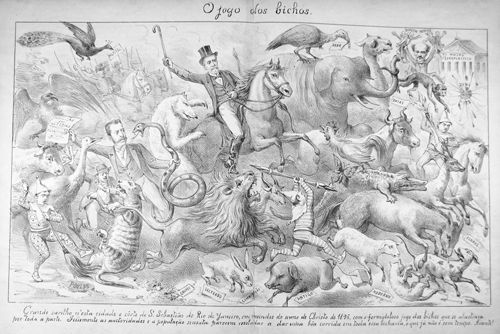
\includegraphics[width=\textwidth, height=6cm]{images/bicho01.jpg}
	\end{minipage}
	\hfill
	\begin{minipage}[b]{0.45\textwidth}
		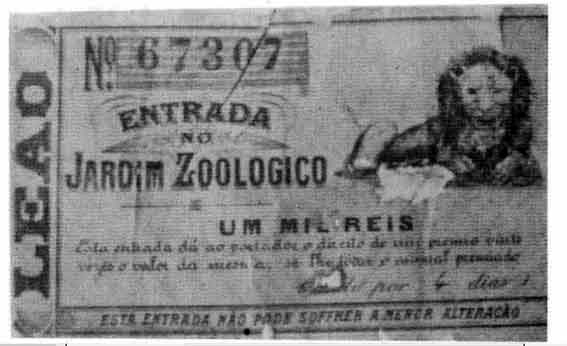
\includegraphics[width=\textwidth, height=6cm]{images/bicho02.jpg}
	\end{minipage}
	\caption{Left: cartoon of the Baron of Drummond and the animals of the \emph{jogo do bicho} (1896). Right: entry ticket to Rio's Zoological Garden that allowed the bearer to join the raffle. Sources: Instituto Histórico e Geográfico Brasileiro, Rio de Janeiro, Revista Illustrada, ano 21, no. 718 (1896) and Museu da Imagem e do Som, Rio de Janeiro. Reproduced in \citet[35--36]{chazkel2011laws}.}
	\label{fig:barao}
\end{figure}

Moreover, the animal game plays a crucial role in the expansion of Rio de Janeiro's Carnival Parade, a popular festivity synonymous with Brazil at home and abroad \citep{araujo2003carnaval,costa2001100,da1973carnaval, da1979carnavais,vianna1995misterio}. \emph{Bicheiros} donate hefty sums to `samba schools' to gather support of poor communities and, no less importantly, to co-opt local politicians attracted by the financial and electoral gains offered by the festival \citep{cavalcanti2006carnaval, queiroz1992carnaval}. This patron-client relationship has been proven effective: in 2016, the Carnival generated about USD 900 million in revenue and the Rio de Janeiro state received more than one million tourists.\footnote{Data provided by the Brazilian government. See \url{https://goo.gl/XMcbTM} (in Portuguese). Access: December 2016.}

In this article I offer a rational choice interpretation of the \emph{jogo do bicho} and discuss how \emph{bicheiros} promote social order, solve information asymmetries, and reduce negative externalities. My analysis discusses three strands of academic literature. First, this work contributes to the scholarship on extra-legal institutions, mainly to the literature on collective action within criminal organisations. For instance, \citet{gambetta1996sicilian} examines the strategies used by the Sicilian Mafia to settle disputes among their members and enforce rules in the areas they exercise control. \citet{leeson2007arrgh,leeson2009invisible,leeson2010pirational} affirms that pirate groups employed hard-to-fake signals to increase the profitability of their operations. \citet{skarbek2011governance,skarbek2012prison,skarbek2014social}, in turn, highlights the role of written and implicit norms in mitigating rent-seeking and coordinating productive activities in California prison gangs. I argue that \emph{bicheiros} have employed reputation strategies and provided club goods to enforce private contracts and foster trust among criminals. Moreover, I also describe how \emph{bicheiros} have developed sophisticated financial mechanisms, such as informal hedging operations and risk-sharing contracts, to prevent predatory behaviour in their community.

Second, this work relates to the literature on repugnant transactions and the relationship between morality and the market \citep{boettke1995morality, roth2007repugnance, sandel2012money, satz2010some, simmel1900geldes, zelizer1979morals}. In the following sections, I claim that the Brazilian elites have attached pejorative meaning to the \emph{jogo do bicho} to constrain the gambling market. I provide evidence that \emph{bicheiros} were aware of this problem, and as a response, they devised a series of rules aimed at reducing the costs associated with repugnance \citep{labronici2014sorteio, magalhaes2005ganhou}. \emph{Bicheiros} have made considerable efforts to increase the levels of trust in the system and distance themselves from other types of illegal activities. Their main tool to increase credibility was costly signalling, that is, the \emph{bicheiros} hoped the public would see them as credible brokers by sacrificing their immediate interests  \citep{gambetta2009codes,kimbrough2015commitment, schelling1960strategy}.

Lastly, this work connects to the literature on state capture, which is among the most important topics in public choice theory \citep{hellman2003seize, rose1978corruption, rose1999corruption, shleifer2002grabbing, tollison1982rent}. More specifically, I use the Brazilian case to illustrate how politicians and civil servants can be co-opted by criminal groups and produce sub-optimal social outcomes. \citet{queiroz1992carnaval} explored why \emph{bicheiros} turned into patrons of the Carnival's samba schools and affirmed that this influence gave them leverage over political authorities. \citet{misse2007illegal} investigated the links between bicheiros and police officers, and suggested that the illegal lottery had been the main cause of police corruption in Rio de Janeiro until the 1970s. In a similar vein, \citet{jupiara2015poroes} analyse the relationship between the \emph{jogo do bicho} and the military regime in Brazil (1964--1985). I supplement this literature by highlighting how asymmetrical information, agency dilemmas, and rent-seeking behaviour offer convincing explanations to the issues presented above. Although those concepts have a long tradition in public choice, scholars have not applied those ideas thus far to understand the dynamics of the \emph{jogo do bicho}. By doing so, I integrate seemingly contradictory historical facts into a single narrative that connects micro-level decisions to macro-level outcomes.

The remainder of this article proceeds as follows. Section \ref{sec:organisation} presents a brief historical overview of the \emph{jogo do bicho}. It describes the necessary conditions for the emergence of the game and presents its basic organisational structure. Section \ref{sec:governance} details the \emph{jogo do bicho}'s governance mechanisms, particularly the strategies employed by vendors to increase trust in markets that operate at the margins of the law. Section \ref{sec:capture} discusses the links between illegal gambling markets, samba schools and the Brazilian state. Section \ref{sec:conclusion3} offers some concluding remarks.

\section{\emph{Jogo do Bicho} as an Emergent Institution}
\label{sec:organisation}

\subsection{Historical Background}
\label{sub:background}

The early history of the \emph{jogo do bicho} is a textbook example of spontaneous order. Spontaneous orders are emergent macro-level phenomena that result from voluntary actions of purposive, self-interested individuals utilising their contextual knowledge \citep{boettke1990theory, boettke2005methodological, hayek1945use, hayek1960constitution, hayek1973law, leeson2008coordination, menger1871grundsatze, polanyi1948planning, polanyi1951logic}. Drummond, the Zoological Garden's original owner, designed the basic framework for the \emph{jogo do bicho}; but independent bookmakers were the ones who popularised the game \citep[77]{magalhaes2005ganhou}. Ticket sellers could quickly respond to market signals and then allocate their products where they were more valuable because of the lack of central coordination. Moreover, competition among sellers fostered innovation, and the \emph{bicheiros} invented new game rules to make the lottery more appealing to their customers \citep[61]{mello1989historia}. In this sense, the animal game is the materialisation of an evolutionary process of entrepreneurial discovery in which the interactions that provided the highest value to consumers were preserved over time \citep{boettke2008gordon, boettke2014entrepreneurship, buchanan1964should, hayek1978competition, kirzner1997entrepreneurial}.

However, the \emph{jogo do bicho} only emerged because of historically contingent circumstances. The late nineteenth-century Brazil had four characteristics that explain how the animal game came to being: 1) a growing urban population excluded from the formal labour market; 2) an inflow of immigrants whose extended family networks helped them engage in trade; 3) an expansion of the monetary supply in the first years of the republic (1880s--1890s); and 4) a judicial system that, albeit repressive, had only imperfect law enforcement. Figure \ref{fig:dag} presents a simple directed acyclic graph (DAG) \citep{pearl2009causality} that shows the relationships between these explanatory variables and the development of the \emph{jogo do bicho}.\footnote{The main purpose of direct acyclic graphs is to graphically display the possible links among the exposure variables, confounders, and outcomes \citep{morgan2014counterfactuals, pearl2009causality}. DAGs are transparent by definition, as all theoretical choices made by the researcher are stated explicitly in the model. Each single-headed arrow in a DAG indicates that the variable at the origin causes the variable at the end of the directed edge. Dashed edges suggest that two variables are jointly dependent on unobserved common causes. There are no assumptions regarding the functional form of the relationships, and unless mentioned otherwise, the arrows represent fully non-parametric associations. Variables between two nodes are mediators, and variables pointed at by two or more factors have multiple causes. They are called \emph{colliders}. For the sake of clarity, errors are assumed independent and often excluded from the graphs. For an accessible introduction to DAGs see \citet[chap. 3--4]{morgan2014counterfactuals} and \citet{pearl2016causal}.}

\begin{figure}[!htbp]
	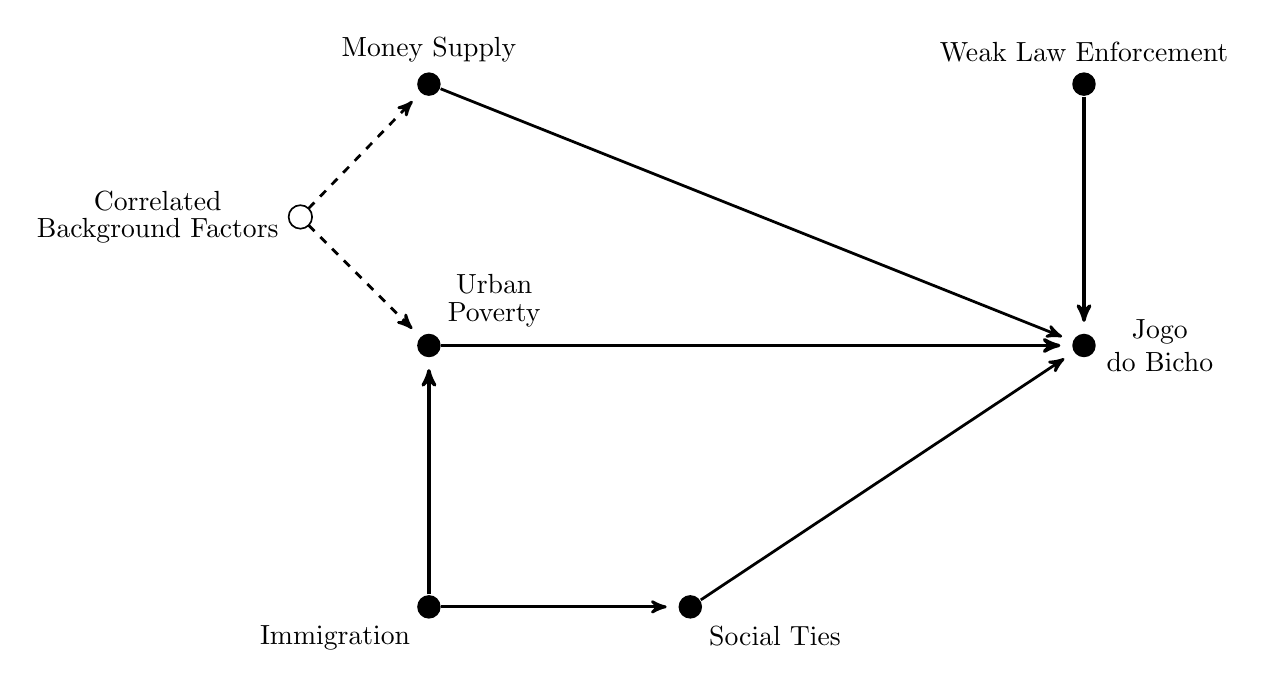
\begin{tikzpicture}[->,>=stealth',shorten >=4pt,auto,node distance=3cm, semithick][h]
		% nodes %
		\node[circle,fill,inner sep=3pt,label=above right: \shortstack{Urban \\ Poverty}] (p) {};
		\node[circle,fill,inner sep=3pt,label=right: \shortstack{Jogo \\ do Bicho}, right = 8 of p] (y) {};
		\node[circle,fill,inner sep=3pt,label=below left: {Immigration}, below = 3 of p] (i) {};
		\node[circle,fill,inner sep=3pt,label=above:{Money Supply}, above = 3 of p] (m) {};
		\node[circle,fill,inner sep=3pt,label=below right:{Social Ties}, right = 3 of i] (s) {};
		\node[circle,fill,inner sep=3pt,label=above:{Weak Law Enforcement}, above = 3 of y] (l) {};
		\node[circle,fill=white, draw, outer sep=0pt, inner sep=3pt,label= left: \shortstack{Correlated \\ Background Factors}, above left = 2 of p] (u) {};
		% edges %
		\draw[->, line width = 1.2] (p) -- (y);
		\draw[->, line width = 1] (s) -- (y);
		\draw[->, line width = 1] (i) -- (s);
		\draw[->, line width = 1.2] (l) -- (y);
		\draw[->, line width = 1] (m) -- (y);
		\draw[->, line width = 1.2] (i) -- (p);
		\draw[->, dashed, line width = 1] (u) -- (p);
		\draw[->, dashed, line width = 1] (u) -- (m);
	\end{tikzpicture}
	\caption{Directed Acyclic Graph -- Explanatory Variables for the \emph{Jogo do Bicho}}
	\label{fig:dag}
\end{figure}

I start with the impact of urban poverty on the animal game. Brazil abolished slavery in the late 1880s, a period in which the country was rapidly urbanising and freed slaves migrated to its growing cities \citep{andrews1991blacks, fausto2014concise, naro1992revision, skidmore1993black}. The former slaves were joined by increasing numbers of Asian and European immigrants \citep{hall1969origins, lesser2013immigration, smith1979ethnic}. Nevertheless, the job market tightened considerably after the \emph{Encilhamento} financial crisis of 1891 \citep{topik2014political, triner2005baring}. During the economic downturn, the informal economy was an obvious destination for the urban poor. Given its widespread popularity, the \emph{jogo do bicho} attracted hopeful entrepreneurs, either Brazilian or foreign-born, who could not enter the formal labour force.\footnote{The underground economy was also more democratic than the formal sector. As \citet[115]{chazkel2011laws} observes, one of the few professions open to poor women and foreigners in the early 1900s was that of street vendor. These vendors used to sell different types of merchandise and many of them would later offer \emph{jogo do bicho} tickets.}

The immigration also influenced the \emph{jogo do bicho} via social ties. Most foreigners who moved to Brazil came from countries, such as Portugal, Spain or Italy, where extended families were the basic form of social organisation \citep{klein1994imigraccao, lobo2001imigraccao, trento1989outro}. Family and neighbourhood networks created incentives for immigrants to establish trade relations and enforce cooperation through community responsibility systems \citep{roth2014prison}. Because of these particular social characteristics, in the 1890s foreigners were over-represented in the Brazilian trade in general \citep{mattos1991vadios, oliveira2001brasil, truzzi2008patricios} and in the \emph{jogo do bicho} in particular \citep{godoi2012imigraccao, magalhaes2005ganhou, torcato2011repressao, villar2008contravencao}. Although kinship bonds became less relevant over time, these links offered an important element of social cohesion in the \emph{jogo do bicho}'s formative years.

Next is the impact of expanded monetary supply. The abolition of slavery and the growing industrialisation of Brazil increased the amount of capital available in the country \citep{franco1987reformas, schulz2008financial}. The 1888 Banking Act gave extra liquidity to local financial markets, and the \emph{jogo do bicho} entrepreneurs utilised that increase in the monetary base to extend the scope of their business. Some years later, the animal game would be available not only across the city of Rio de Janeiro but throughout Brazil \citep[76]{da1999aguias}.

The country's lax financial policy might correlate with poverty through unspecified factors. For instance, political decisions may have caused inadvertently both poverty and the expansion of the monetary base \citep{mattos2013shantytown, schmidt1982modernization}; alternatively, external events such as institutional instability \citep{costantini2014index, fausto2014concise, luna2014economic} or commodity shocks \citep{musacchio2014colonial} could be the cause of those two variables. There is not enough evidence to discard such scenarios. To illustrate this uncertainty, the two nodes, namely, money supply and urban poverty, are connected with a dashed edge in Figure \ref{fig:dag}.

The last necessary condition for the emergence of the \emph{jogo do bicho} is weak law enforcement. \citet[69--100]{chazkel2011laws} notes that until the 1940s police district chiefs operated within a large margin of discretion and repression against bookmakers was idiosyncratic. Prosecution against the \emph{bicheiros} had hardened in 1917, but only in 1946, when the federal government banned all gambling activities in the country \citep[155--156]{magalhaes2005ganhou}, the law was consistently enforced.

\subsection{Organisational Structure}
\label{sub:organisation}

The animal game has three levels of hierarchy. At the bottom are the \emph{bicheiros}, who are those in charge of selling \emph{jogo do bicho} tickets \citep{chazkel2007beyond, chazkel2011laws, da1999aguias, labronici2014sorteio, magalhaes2005ganhou, misse2007illegal}. \emph{Bicheiros} are the most visible part of the \emph{jogo do bicho} structure. The bookmakers often build their vending stands inside the premises of a local shop, such as a small grocery store or a pub, and are recognisable by their chairs facing the street, stamps and blocks of paper \citep[259]{chazkel2011laws}. \emph{Bicheiros} usually work alone, but they may employ up to 10 people depending on how busy their betting site is \citep[69]{labronici2014sorteio}.

The \emph{gerentes} (managers) oversee all \emph{jogo do bicho} stands in a given area. Their task is akin to that of a firm accountant. Gerentes control the cash flow between the \emph{bicheiros} and the bankers, manage the payroll of the employees, and provide financial information to the top members of the organisation. They also supervise individuals who carry menial tasks in the business, transfer money to other gambling branches and double-check the balance sheets of the betting sites \citetext{\citealp[71]{labronici2012paratodos}; \citealp[142]{misse2007illegal}}.

\begin{figure}[!htbp]
	\centering
	\begin{minipage}[b]{0.45\textwidth}
		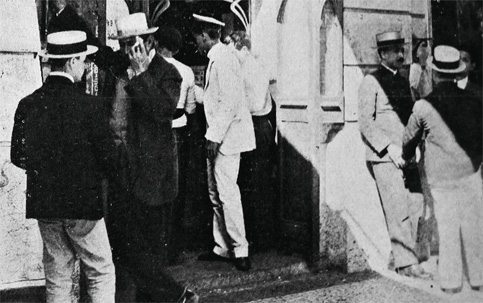
\includegraphics[width=\textwidth, height=6cm]{images/bicho03.jpg}
	\end{minipage}
	\hfill
	\begin{minipage}[b]{0.45\textwidth}
		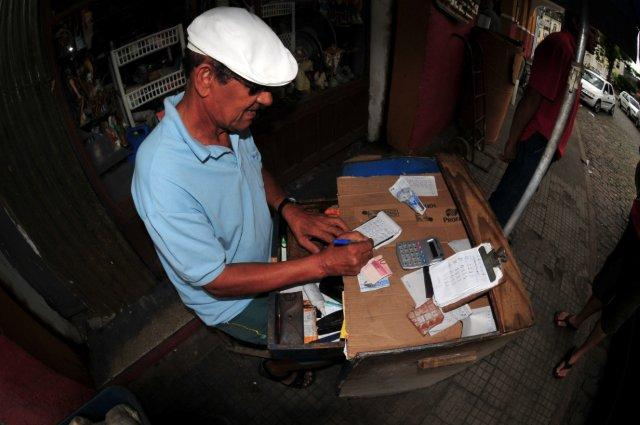
\includegraphics[width=\textwidth, height=6cm]{images/bicho04.jpg}
	\end{minipage}
	\caption{\emph{Jogo do bicho} betting sites in 1917 and in 2011. The picture on the right shows a \emph{bicheiro}, a street-corner vendor. Sources: \citet{alecrim2012bicho} and \citet{ferrarini2011bicho}.}
	\label{fig:banca1917}
\end{figure}

The \emph{banqueiros}, or the Portuguese for bankers, occupy the top position in the \emph{jogo do bicho} hierarchy, comprising the small financial elite of the game. A 2012 report by the Brazilian Federal Police affirmed that 10 \emph{banqueiros} controlled the market throughout the country; five of them based in the state of Rio de Janeiro \citep{globo2012contraventores}. Apart from funding the game, the bankers provide support for the employees to undertake their activities. The \emph{banqueiros}' main attributions include paying bribes to police personnel, bailing out sellers arrested by security forces, and offering judicial assistance to employees in case of legal persecution \citep[75]{labronici2012paratodos}.

\emph{Banqueiros} run their businesses from fortified houses in unknown locations, the \emph{fortalezas} (`forts'). The first \emph{fortalezas} likely appeared in the 1950s, when the animal game was already well-established across the Brazilian territory. The period coincides with a time when the \emph{jogo do bicho} finances had become increasingly concentrated in fewer hands \citep[259]{chazkel2011laws}. Due to the growing size of the \emph{jogo do bicho} economy, \emph{banqueiros} decided to move their operations away from the public to avoid police persecution and reduce coordination costs.

Although the forts provided safety to the bankers, the existence of those hideouts posed a challenge to the organisation. Bankers removed from the public view are not accountable to players and booking agents. Similarly, bankers and managers working in the \emph{fortalezas} cannot oversee their employees as effectively as before. Considering that the animal game itself is illegal and the amount of money involved in the bets is often substantial, both \emph{banqueiros} and booking agents have strong incentives to defect. Players, in turn, have no evident reason to trust \emph{banqueiros} or \emph{bicheiros}. How do \emph{jogo do bicho} agents overcome trust issues and cooperate under uncertainty?

I argue that the \emph{jogo do bicho} solves problems of internal cooperation by providing club goods \citep{buchanan1965economic, berman2008religion, berman2009radical, leeson2011government, roth2014prison} while simultaneously shunning cheaters through punishments and appeals to `the shadow of the future' \citep{axelrod1984evolution, axelrod1985achieving, bo2005cooperation, roth1978equilibrium}. Clients and \emph{bicheiros} cooperate based on trust-enhancing mechanisms, most of them devised specifically for the \emph{jogo do bicho} \citep{da1999aguias, magalhaes2005ganhou}. Such mechanisms are relevant because they have allowed the \emph{jogo do bicho} to distance itself from other shadow markets and become a profitable enterprise in the long run.

\section{Governance of the \emph{Jogo do Bicho}}
\label{sec:governance}

\subsection{Gambling Markets and Repugnant Transactions}
\label{sub:repugnance}

The \emph{jogo do bicho} is a repugnant market. Individuals that like to gamble cannot do so because of strong moral objections from outsiders \citep{brisset2016marche, roth2007repugnance, satz2010some, zelizer1979morals}. As early as in 1890, Brazilian public authorities positioned themselves against the \emph{jogo do bicho} arguing that `{[}\ldots{}{]} this type of amusement is prejudicial to the interests of the unwise, who are naively seduced by the deceptive hope of uncertain lucre' \citep[544]{chazkel2007beyond}. In 1941, the government banned the animal game;\footnote{See: \url{http://www.planalto.gov.br/ccivil_03/decreto-lei/Del3688.htm} (in Portuguese). Access: December 2016.} five years later, it prohibited all games of chance.\footnote{The 1946 decree stated that gambling was `harmful to morality and the good customs', hence `[\dots] the repression against games of chance [was] an imperative of the universal consciousness'. The text can be read at: \url{http://www.planalto.gov.br/ccivil_03/decreto-lei/Del9215.htm} (in Portuguese). Access: December 2016.} The \emph{jogo do bicho}, casinos and bingos remain illegal in the country. Recent estimations show that the prohibition of the \emph{jogo do bicho} have prevented the state from earning BRL 15 to BRL 20 billion (USD 4.5 to USD 6 billion) per year in expected taxation revenues, aside from the subjective utility losses for players. \citep{congressoemfoco2015bicho, fsp2016legalizarbicho}.

In contrast with the official statements, the noxious element of the \emph{jogo do bicho} does not come from its inherent randomness. The game is `repugnant' precisely because it is \emph{a market}, a setting in which individuals can monetise the entertainment for private profit \citep{chazkel2007beyond, chazkel2011laws}. The Brazilian state has never seen any contradiction between banning games of chance and running a national lottery company of its own; even the Catholic Church, which has long condemned the \emph{jogo do bicho}, frequently organises raffles to fund its activities \citep[49]{abreu1996imperio, magalhaes2005ganhou}. Only after the introduction of private money that Brazilians objected the idea of benefiting from someone else's bad luck.

In this sense, the main obstacle that confronted \emph{bicheiros} was to convince others that the animal game would not cause the Brazilian society `to slide down a slippery slope to genuinely repugnant transactions' \citep[45]{roth2007repugnance} such as prostitution or debt bondage. As the century-old history of the game can attest, \emph{bicheiros} have succeeded in this task. But how? The literature on repugnant costs tell us little about how markets transition from noxious to tolerated. Here I posit two mechanisms that reduced the stigma associated with the game: 1) \emph{a strong reputation of honesty} expressed by costly signals from sellers, and 2) the provision of \emph{selective incentives} for both clients and booking agents. Below, I offer evidence that these two factors allowed the animal game to reach its current semi-legal status in Brazil.

\subsection{External Cooperation}
\label{sub:external}

Evolutionary game theory \citep{axelrod1984evolution, axelrod1985achieving, smith1982evolution} and experimental studies \citep{dawes1977behavior, isaac1984divergent, kim1984free, marwell1981economists} have both demonstrated that long-term cooperation is possible whenever players expect future pay-offs to be higher than present ones. Fear of retaliation induces individuals not to cheat. Nevertheless, illegal organisations tend to discount the future even more heavily than the other groups, what makes cooperative behaviour among criminals uncommon \citep{gambetta2009codes, skarbek2011governance,skarbek2012prison,skarbek2014social}. The \emph{jogo do bicho} is an exception to this rule. The market properties of the game and inconsistent repression by Brazilian authorities have permitted \emph{bicheiros} to overcome the stigma of repugnance and improve the game's long-term profitability.

The \emph{jogo do bicho} entrepreneurs have made considerable efforts to present themselves as honest brokers. The first trust-enhancing mechanism they have employed to foster external cooperation was the use of a \emph{fixed-multiplier formula} for pay-outs. It works as follows. If a player wins the lowest prize of the animal game, he or she receives 18 times his/her investment regardless of the size of the bet. Bigger prizes naturally offer higher returns; a lucky winner of the top prize wins up to 4,000 times the value of his/her bet \citetext{\citealp[89]{labronici2012paratodos}; \citealp[20]{magalhaes2005ganhou}}.

This stands in sharp contrast to the common practice of sharing a prize among winners. Lottery pay-outs demand high levels of interpersonal trust: players rely on unverifiable information about the total funds collected by the lottery, and they can never be sure whether the payments are evenly distributed. The fixed-multiplier formula alleviates such problems of adverse selection \citep{akerlof1970market, cohen2010testing, levin2001information}. As players and vendors known the prize value beforehand, the method provides consumers with complete information about their individual prizes while also binding the \emph{bicheiros} to a contract that can be easily enforced. This technique offers buyers a simple yet effective screening strategy that induces \emph{bicheiros} to provide honest information about the game \citep{spence1973job, stiglitz1981credit}.

\emph{Bicheiros} have addressed information asymmetries in another ways. Since the 1950s, when the \emph{jogo do bicho} bankers had moved their operations to the \emph{fortalezas}, the public could not oversee the lottery draws \citep[259]{chazkel2011laws}. This could lead to a decline in trust among buyers and vendors of lottery tickets and, as a result, to reduced profits. \emph{Bicheiros} have mitigated this problem with a two-pronged strategy. First, they started to utilise the winning numbers from the licit government-run lottery, the \emph{Loteria Federal}, instead of their own draws \citetext{\citealp[546]{chazkel2007beyond}; \citealp[89]{labronici2012paratodos}; \citealp[39-40]{mello1989historia}}. The federal lottery numbers are public information. The media broadcasts the draws on radio and TV, so any interested player can verify the selected numbers. The Loteria Federal is also audited by two independent state institutions, a private accounting firm, and voluntary members of the public; hence, \emph{bicheiros} can free ride on the lottery's long-standing reputation of credibility.\footnote{As of April 2016, the lottery was audited by the \emph{Controladoria Geral da União} (Comptroller General of Brazil), the \emph{Tribunal de Contas da União} (General Accounting Office), and by Ernst \& Young. The balls are measured and weighted every three months by the National Institute of Metrology, Quality and Technology (Inmetro), the Brazilian equivalent of United Kingdom's National Physical Laboratory or the American National Standards Institute. See \url{http://noticias.uol.com.br/cotidiano/ultimas-noticias/2016/04/08/auditoria-dos-sorteios-da-caixa-e-confiavel-veja-como-e-o-processo.htm} (in Portuguese). Access: December 2016.}

\begin{figure}[!htbp]
	\centering
	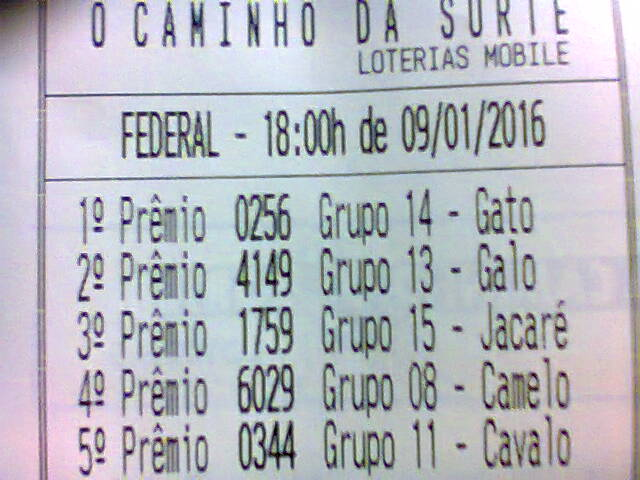
\includegraphics[width=\textwidth, height=6cm]{images/bicho06.jpg}
	\caption{Results of a \emph{jogo do bicho} draw from 09 January 2016. `Federal' means that the winning numbers were drawn by the federal government lottery. The first prize was group 14, the cat. Source: Unknown. Available at: \url{https://goo.gl/6PHV8u}. Access: December 2016.}
	\label{fig:federal}
\end{figure}

Second, they included representatives of all major \emph{jogo do bicho} bankers in every draw and independently publicise the game results. Certain \emph{bicheiros} went as far as publishing the numbers in Rio's newspapers. In the early twentieth century, some tabloids were entirely dedicated to the game \citep[60]{magalhaes2005ganhou}. Booking agents see this strategy as a credible signal from the game financiers, as providing contrasting information would indicate game manipulation. Moreover, collusion can also be spotted if the draws show repeated numbers or unusual patterns.

\begin{figure}[!htbp]
	\centering
	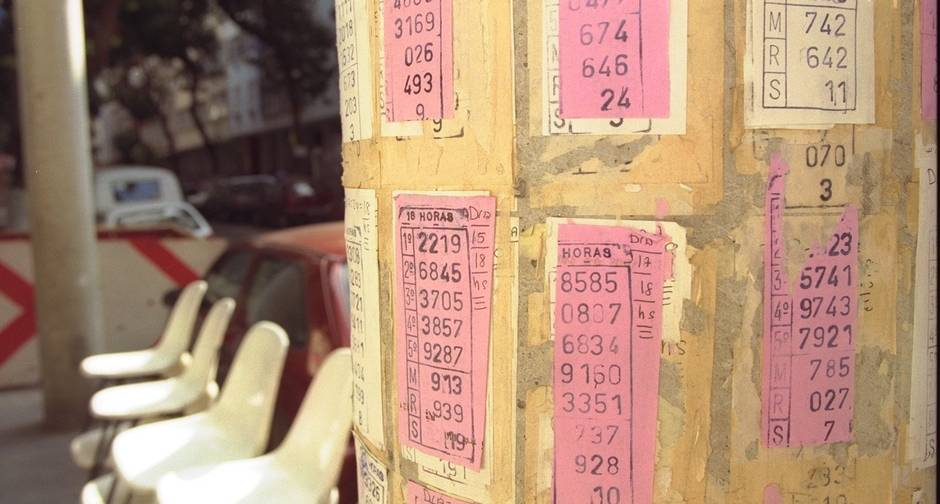
\includegraphics[width=\textwidth, height=6cm]{images/bicho05.jpg}
	\caption{\emph{Jogo do bicho} results are fixed on light poles in Rio de Janeiro. Source: \citet{gomes1998bicho}.}
	\label{fig:poste}
\end{figure}

These efforts have proved popular with the game enthusiasts. One often-repeated saying about the \emph{jogo do bicho} is that `in the \emph{jogo do bicho}, what is written down counts' \citep[159]{chazkel2011laws}, that is, buyers and sellers do fulfill their informal obligations without third-party enforcement. Such mutual confidence reduces the potential for conflict in the game. As the public does not see the \emph{jogo do bicho} as violent or harmful, the stigma of repugnance associated with gambling becomes less pervasive. By reducing the possibilities of cheating and putting long-term interests first, the \emph{jogo do bicho} bankers have avoided the fate of other repugnant markets and run their business relatively undisturbed for decades \citep[20]{da1999aguias}.

\subsection{Internal Governance}
\label{sub:internal}

Individuals working at different levels of hierarchy often have non-aligned interests. As a result, it may occur that one party (the agent) behaves rationally in a manner that maximises his/her benefits, but that is contrary to the interests of his/her superior (the principal). This dilemma is pervasive in formal organisations \citep{holmstrom1979moral,jensen1976theory,moe1984new,shapiro2005agency,spence1971insurance}; in illegal markets perhaps it is even more so \citep{campana2013cooperation,gambetta2009codes,skarbek2011governance,skarbek2014social}. As monitoring costs in criminal businesses are higher than in formal ones, principals face considerable difficulties to induce cooperation from agents. Moreover, criminals often engage in opportunistic behaviour and `hidden actions', that is, they do not put the required levels of effort if they know they are not being monitored \citep[38--42]{arrow1985agency}.

In the \emph{jogo do bicho} setting, one such problems concerns the trade-off between short- and long-term incentives for managers and bankers on the one side and bookmakers on the other. Managers have a permanent interest in the long-run profitability of the game, whereas street-corner booking agents tend to discount the future more heavily because their financial gains are small compared to that of their superiors. Additionally, bookmakers may denounce their employers to the police if they feel threatened.

One way by which the \emph{jogo do bicho} principals solve the agency dilemma is by supplying club goods and selective incentives for low-tier members. Club goods are goods that can be simultaneously enjoyed by more than one individual but where exclusion mechanisms prevent consumption by non-members \citep{buchanan1965economic, cornes1996theory, olson1965logic, sandler1980economic, sandler1997club}. Basically, club goods are `public goods \emph{sans} non-excludability' \citep[928]{mcnutt1999public}. The first club good offered to \emph{bicheiros} by their bosses is private security. The game bankers have built an extensive network of gunmen and bribed police officers to protect their employees (and their profits) from other criminals \citetext{\citealp[48]{chinelli1993vazio}; \citealp[51]{labronici2012paratodos}}. The \emph{jogo do bicho} network has a powerful deterrence effect and lethal force is rarely employed. However, threats are constant. `Zé' (Little Joe), a bicheiro interviewed by \citet[52]{labronici2012paratodos}, described eloquently the deterring effect of the \emph{jogo do bicho} informal security personnel:

\begin{quote}
	[\dots] bums are scared and they don't mess around with us; they think there's a guard nearby or something like that. Look at all this money here! [shows the interviewer a handful of cash] It's not ours [referring to street-corner bookmakers]. And if it's not ours, it's someone else's. When I worked in Penha (\emph{a low middle-class neighbourhood in the city of Rio de Janeiro -- translator's note}), the owner of a pub close to where I used to work always asked me to stay at the front door of his pub. People know that bums are afraid of \emph{bicheiros}.
\end{quote}

Apart from guaranteeing the physical integrity of the \emph{bicheiros}, bankers and managers also provide financial incentives for the bookmakers. \emph{Bicheiros} are allowed to receive tips from players, often have small expenses paid by managers, and may even request interest-free loans to cover unexpected costs such as illness-related expenses \citep{labronici2012paratodos}.

However, the most important financial mechanism implemented by bankers to help \emph{bicheiros} is the \emph{descarga}, which is loosely translated as `the unloading'. The descarga is the \emph{jogo do bicho}'s main hedging technique and its purpose is to insure bookmakers against credit risk \citetext{\citealp[59]{labronici2012paratodos}; \citealp[178]{magalhaes2005ganhou}; \citealp[16]{misse2007illegal}; \citealp[75]{soares1993jogo}}. Booking agents are sometimes unable to honour expensive bets. As mentioned above, the top prize in the animal game pays up to 4,000 times the amount invested, thus \emph{bicheiros} may have to raise thousands of Brazilian Reals in a single day. To prevent the \emph{quebra da banca} (`bust of the bank'), \emph{bicheiros} and small bankers buy an insurance from wealthier financiers, who offer this service for a fee that ranges from 20\% to 25\% of the total selling amount \citep{fsp2006descarga}. The \emph{descarga} guarantees that small bookmakers will not have liquidity problems, thus permitting bookmakers to continue investing in the \emph{jogo do bicho}.

The descarga has played an important role in reducing individual risk; nevertheless, it has also changed the distribution of resources in the \emph{jogo do bicho}. Simple probability dictates that a booking agent rarely pays the highest prize in the \emph{jogo do bicho}; in contrast, the bankers receive a commission for \emph{every game} they hedge. Over time, there is a transfer of income from the bottom to the top of the animal game structure led by this constant inflow of fees. This accumulation of capital is probably one of the reasons why bankers were able to diversify their businesses and offer other types of entertainment such as slot machines and sports lotteries \citep{estado2006cacaniquel,globo2015cacaniquel,terra2011cacaniquel}. The descarga has made the game more resilient at the aggregated level, although it increased profits for the richest financiers at the expense of small bookmakers.

\section{Tropical State Capture: \emph{Jogo do Bicho}, Samba and Politics}
\label{sec:capture}

The impact of the \emph{jogo do bicho} is not restricted to the Brazilian economy. Since the 1960s, \emph{bicheiros} have been the key sponsors of the country's most important cultural and social festivity, the Rio de Janeiro Carnival parade \citep{bezerra2009mecenato,cavalcanti2006carnaval,chinelli1993vazio,queiroz1992carnaval}. The \emph{jogo do bicho} accounts for such large share of the funding of the parade that a famous \emph{banqueiro} once remarked that `without the \emph{jogo do bicho} the Carnival would have ended' \citep{odia2016aniz}. Owing to that support, \emph{bicheiros} have established an extensive patronage network with samba schools and local politicians \citetext{\citealp[4641]{arguello2012criminalizaccao}; \citealp{congressoemfoco2007bicho}; \citealp{jornaldobrasil2011bicho}; \citealp[16]{misse2011crime}}. Although that network brings large material benefits to their members, the patronage system has created perverse incentives for government officials.

The \emph{jogo do bicho}'s clientelism is more evident in the state of Rio de Janeiro than in other parts of the country. Historical factors explain why this is the case. Firstly, Rio de Janeiro city was the capital of Brazil for almost 200 years; despite losing the position to Brasília in 1960, it remains one of the country's main cultural and financial centres. Secondly, \emph{jogo do bicho} operators had historical ties with popular movements, which they eventually exploited to their advantage. Thirdly, the emergence of state-sponsored Carnival parades created a window of opportunity for \emph{bicheiros} to expand their influence over public authorities, either via bribing or by funding political campaigns. In this regard, Rio provided a suitable environment for self-interested politicians, community leaders and animal game financiers to collaborate. These illegal networks are crucial to understand why samba and Carnival became constituent features of Brazil's national identity, and how the festival has contributed to Rio's high levels of state corruption.

\subsection{The `Medici of Samba': \emph{Bicheiros} as Patrons of Carnival}
\label{sub:patrons}

In 1930, opposition leader Getúlio Vargas led a bloodless coup d'état that brought Brazil's First Republic to an end. During his first presidency (1930--1945), Vargas promoted a radical shift in Brazilian politics by dismantling effectively federalism in favour of a powerful executive branch and an expanded federal bureaucracy \citep[e.g.][]{bethell2008politicsvargas,desouza1983estado,fausto1972revoluccao,fausto2014concise,skidmore1967politics}. In terms of ideology, Vargas's authoritarian-corporatist \emph{Estado Novo} (``New State'') promoted a politicised nationalism designed to transcend the regional aspects of Brazilian culture \citep{lauerhass1972getulio,nava1998lessons,williams2001culture}. Popular music, in turn, occupied an important place in Vargas's project of `brazilianing Brazil'. Created in the late 1920s in the shanty towns of Rio de Janeiro, modern samba embodied the idea of the multicultural, racially-tolerant country the government aspired to forge \citep{avelar2011brazilian,mccann2004hello,stockler2011samba,vassberg1969villa,vassberg1975villa}.

By the late 1930s, samba reached a unique position in Brazil's cultural identity. In a period when civil and political rights were limited \citep{de2001cidadania,duarte1993vicissitudes}, Vargas used samba as a means to incorporate ethnic minorities and the new urban classes into the Brazilian mainstream \citep[213]{chinelli1993vazio}. Patriotic sambas exalted the country's natural beauties and the figure of the `friendly, happy, cordial and industrious' mulatto\footnote{A mulatto is a person of mixed white and black ancestry. The etymology of the word is originally derogatory as it alludes to `mule' (Latin: \emph{mulus}), the infertile offspring of the male donkey and a female horse. However, in the 1930s the word loses its pejorative connotation in Brazil. Mainly due to the work of sociologist \citet{freyre1933casa}, the idea of a racial democracy becomes pervasive in the government discourse, and as a result the word gains a positive tone \citep[4]{reiter2009brazil}.} \citetext{\citealp[47]{dangelo2016samba}; \citealp[51]{vianna1995misterio}}. The institutionalisation of the Carnival parade in 1935, and the subsequent increases in public funding to the festival, cemented the relationship between politicians and samba groups \citep{almeida2017carnaval,cabral2016escolas,soihet1998subversao}.

However, the samba groups were not passive members in this process. Since the 1960s, the Rio Carnival expanded in scope and, stimulated by growing numbers of spectators, the parades became more elaborate \citetext{\citealp{cabral2016escolas}; \citealp[214]{chinelli1993vazio}; \citealp[240]{hertzman2013making}}. Unable to cope with the rising costs of the show, the `samba schools', which are large samba groups that compete in the Carnival, resorted to the \emph{jogo do bicho} financiers to fund their activities \citep{misse2007illegal}. This informal agreement between samba school organisers and wealthy \emph{bicheiros} remains effective to this day, and many of Rio's most famous samba schools are officially presided by high-profile members of the \emph{jogo do bicho} elite \citep{bezerra2009mecenato,cavalcanti2006carnaval,farias2013carnival,misse2011crime,queiroz1992carnaval}.

As I have mentioned in the previous section, the animal game at times faced opposition by the local population. The public often perceived the game as immoral and repugnant. Moreover, even after the bicho was well-established in Rio de Janeiro, the transition from a competitive betting market to an oligopoly involved the threat and often the use of physical violence against bookmakers who resisted the change \citetext{\citealp[143]{bezerra2009mecenato}, \citealp[52]{labronici2012paratodos}}. \emph{Bicheiros} were aware of the reputation costs their strategy entailed. They decided to finance samba schools hoping to win `the hearts and minds' of the population and attach a more positive image of the game among urban classes. Members of the \emph{jogo do bicho} had been involved in the Carnival since the early 1920s, but only as individuals who had a private interest in samba \citep[209]{chinelli1993vazio}. In 1984, a group of rich \emph{jogo do bicho} financiers founded collectively the LIESA (\emph{Liga Independente das Escolas de Samba}, Independent League of the Samba Schools), a civil association intended to direct and sponsor the Carnival parade in Rio de Janeiro. The LIESA marked a shift in the Carnival. For the first time, \emph{bicheiros} decided to act as a group rather than individuals. The organisation consolidated the power of \emph{bicheiros} over the parade and provided a formal mechanism to solve disputes among the samba school patrons \citetext{\citealp[43]{cavalcanti2006carnaval}; \citealp[171]{farias2013carnival}; \citealp[55]{labronici2012paratodos}}.

\begin{figure}[!htbp]
	\centering
	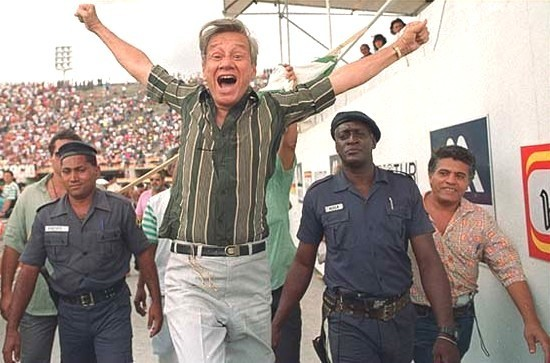
\includegraphics[width=.8\textwidth, height=8cm]{images/bicho07.jpg}
	\caption{Castor de Andrade is shown celebrating after the samba school he sponsored, Mocidade Independente, won the Carnival parade in 1996. He was surrounded by colleagues and police officers. Andrade was the founding president of LIESA (1984--1985) and the wealthiest \emph{bicheiro} of Rio de Janeiro at the time. Source: Folha Imagem. Reproduced in \citet[139]{misse2007illegal}.}
	\label{fig:castor}
\end{figure}

The funding of the samba schools had an indirect effect to the animal game. The patronage also reduced agent-principal problems within the \emph{jogo do bicho}. \emph{Bicheiros} donate to samba school to gather support of the communities, and by doing so they gain access to local information on their business. Clients who have a positive image of the \emph{bicheiro} may denounce fraudsters to their superiors, thus monitoring is cost-effective for animal game managers. Thus, street bookmakers have fewer incentives to cheat. In addition, street sellers are often recruited from the poor communities, so they tend to be immediate beneficiaries of \emph{bicheiros}'s donations \citep{bbc2012aniz}. Hence, funds donated to samba schools and other charities organisations help align the interests of different members of the \emph{jogo do bicho} organisation. The patronage can be interpreted as an illegal version of `profit-sharing', a mechanism which has induced effectively cooperative behaviour in both small and large corporations \citep{cahuc1997profit,fitzroy1987cooperation, kruse1992profit}.

The samba schools have profited from this association too. First, they have gained autonomy from the government. The samba schools do not need to rely exclusively on public funds to organise the parade, and money from the \emph{jogo do bicho} permitted the schools to act independently \citep[209]{chinelli1993vazio}. Second, the support of the \emph{jogo do bicho} has increased the political and social clout of the samba schools. In a country where the state is not present throughout the territory and human right abuses are frequent \citep{ahnen2003,odonnell1993state,pinheiro2000,pinheiro2001}, \emph{jogo do bicho} bankers, and more recently drug traffickers, have provided private governance to poor areas of Rio de Janeiro by enforcing property rights, mediating disputes, and preventing police abuse in the favelas \citep{arias2006dynamics,goldstein2013laughter,leeds1996cocaine}. In return for funds and protection from the \emph{bicheiros}, samba schools have served as intermediaries between the underworld and the political system. Although the \emph{banqueiros} are interested in weak law enforcement against the animal game, politicians have resorted to samba schools to contact \emph{bicheiros} and use their financial and electoral influence in the shanty towns \citep[17]{misse2011crime}. The samba schools, therefore, have increased their bargaining power in the political sphere and extended their reach within Rio's poor communities \citep[215]{chinelli1993vazio}.

\subsection{Political Support}

If politicians were opposed to the \emph{jogo do bicho} in the early twentieth century, their relationship with the animal game bankers have become more ambivalent in the last decades. The collaboration between public authorities and \emph{bicheiros} gained prominence during the military dictatorship (1964--1985) \citetext{\citealp{gaspari2002ditadura}; \citealp{jupiara2015poroes}; \citealp[39]{zaluar2007democratizaccao}}. Given the absence of democratic checks and balances, paramilitaries and police forces colluded to repress potential dissidents of the regime and, frequently, to extort civilians \citep{gorender1999combate,magalhaes1997logica,misse2009acumulaccao,skidmore1990politics}. \emph{Bicheiros} saw the corruption of some members of the military as an opportunity. Wealthy \emph{jogo do bicho} bankers hired rogue police officers not only to work as security guards but to threaten eventual competitors in their regions of influence. The agreement between \emph{bicheiros} and corrupt members of the military was the ultimate responsible for the transformation of the \emph{jogo do bicho} into a `coercive oligopoly' \citep{jupiara2015poroes}. The support of the armed forces meant that new groups would be prohibited from entering the market and that the illegal lottery could operate undisturbed by the government.

The links between \emph{bicheiros} and the public authorities changed after Brazil became a democracy in 1985. In the military regime, government officials were mainly interested in bribes from the animal game. But in the democratic period, votes became a sought-after political resource. \emph{Bicheiros} are important in this sense as they have direct influence over a number of poor communities. Their patronage networks ensure that candidates supported by \emph{bicheiros} receive a substantial amount of votes from areas where campaigning is too difficult or too costly \citep[17]{misse2011crime}.

The Brazilian political system is particularly conductive to clientelistic practices. Brazil has one of the most fragmented party systems in the world, which induces political entrepreneurs to run highly individualised campaigns \citep{figueiredo2000presidential,geddes1992institutional}. In addition, Brazil uses a open-list proportional representation electoral system, that is, each of the 27 states of the federation are considered as at-large electoral districts \citetext{\citealp{ames1995electoral}; \citealp{mainwaring1992brazilian}; \citealp[483]{samuels2000ambition}}. These two elements indicate that Brazilian politicians are often free from the strong requirements of political parties and can run their campaigns with a high degree of independence. Nevertheless, that independence means candidates rely mostly on themselves to raise funds and establish communication with potential voters. Hence, political campaigns in Brazil tend to be expensive and personality-centred.

The support from the \emph{jogo do bicho} mitigates both problems. With respect to the financial costs of campaigns, illegal donations from \emph{bicheiros} help to cover advertising expenses while having the additional benefit of not appearing in the official records of the candidates \citep{congressoemfoco2007bicho,gazetadopovo2007bicho,globo2012bicheiro}. This suggests that \emph{jogo do bicho}-funded politicians can circumvent spending limits and have an electoral advantage over their competitors. As candidates do not know whether their competitors receive funding from the \emph{jogo do bicho} nor the amount each one was paid, their dominant position is to contact the \emph{bicheiros} and join their networks. The situation is a prisoner's dilemma in which candidates would be better off by running cheaper campaigns and not being dependent of \emph{jogo do bicho} bankers, but asymmetric information prevents them from reaching an optimal solution.

\begin{figure}[!htbp]
	\centering
	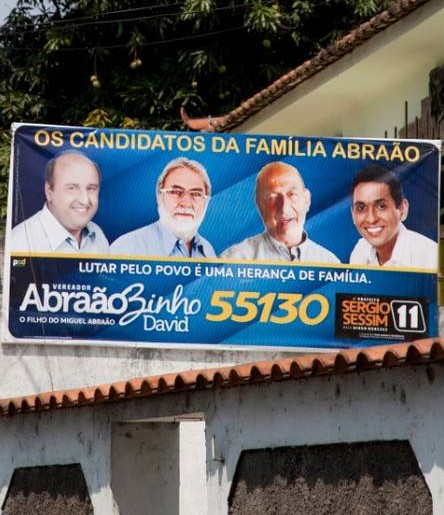
\includegraphics[width=.6\textwidth, height=8cm]{images/bicho08.jpg}
	\caption{Political advertising for Abraãozinho David (right), nephew of the \emph{jogo do bicho} banker Aniz Abraão David (third from left to right). The banner reads: `The Candidates of the Abraão Family: Fighting for the People is a Family Heritage'. Source: \citet{extra2012aniz}.}
	\label{fig:aniz}
\end{figure}

The votes from poor communities are instrumental for aspiring politicians. Brazil has an enforced compulsory voting system; therefore, turnout rates tend to be higher than in other democracies. Consequently, votes have high marginal utility for politicians. As elections may be decided by a small difference, the \emph{bicheiros}' clientelistic ties guarantee a minimum number of votes that politicians can rely upon on election day. Nonetheless, the patronage subverts the preferences of the public and, as such, the democratic process per se. Individuals may be punished if the candidate does not receive the expected number of votes, and are often compelled to vote for politicians that have only loose connections with their communities. Therefore, although voters have the right to choose their representatives, in practice the suffrage is limited for a share of Brazil’s lower classes.

Finally, the \emph{jogo do bicho} patronage highlights a crucial social dilemma within the Brazilian public law. Even though federal judges have prosecuted \emph{bicheiros}, politicians and police forces have no incentives to enforce the punishment. Although Brazilian judges enjoy job stability, the latter groups constantly require local-level support from the \emph{bicheiros}. Politicians and police officers may have accurate information on \emph{jogo do bicho} operations and \emph{bicheiros}' whereabouts, but the federal government cannot rely upon their cooperation. That can be one of the reasons why even after many attempts to arrest \emph{bicheiros}, there has been little progress in that regard in Brazil's latest democratic period (1985--present).

\section{Conclusion}
\label{sec:conclusion3}

Past research has shown that criminal organisations face considerable challenges to elicit cooperation from their members and establish close ties with the population \citep[e.g.][]{gambetta1996sicilian,skarbek2011governance,skarbek2012prison,varese2001russian,varese2011mafias}. Yet, the \emph{jogo do bicho} offers a convincing example that it is possible for an illegal syndicate to operate with low levels of violence for more than a hundred years. \emph{Bicheiros} employ a number of strategies to obtain reliable information from their subordinates while offering club goods and other selected benefits to workers. Furthermore, by investing in the Carnival parade \emph{bicheiros} have been able to gather popular and government support. Poor communities have associated with the \emph{bicheiros} to receive welfare provision, whereas politicians have collaborated with them to reap the financial and electoral benefits the \emph{jogo do bicho}'s networks can provide.

Nevertheless, the \emph{jogo do bicho} has also created negative externalities. Violence is used to punish defectors and to constrain competitors. The clientelistic relationship that \emph{bicheiros} have with local politicians have lead to sub-optimal outcomes, such as predatory political campaigning, distortions in electoral representation, and impunity for human rights violations. These negative externalities have long-term effects and still impact the Brazilian public sphere.

Although the \emph{jogo do bicho} has received an increasing attention from scholars, much of its inner workings remain poorly understood. First, the relationship between \emph{bicheiros} and drug dealers is a topic that deserves attention. Brazil has become one of the world's largest consumers of illicit drugs and South America's principal drug trafficking transit route \citep{miraglia2015drugs,misse2011crime}. The question whether \emph{bicheiros} collaborated or opposed the emergent drug dealing business is still unclear. Second, the extent to which \emph{bicheiros} use other businesses, such as hotels or factories, to laundry money has been mentioned by members of the Brazilian judiciary \citep{globo2012bicheiro,globo2015cacaniquel}; however, there is no reliable estimate on its size. Lastly, more research is required to clarify how \emph{bicheiros} from different parts of Brazil coordinate their activities and prevent large-scale conflicts. Cases studies are usually focused on Rio de Janeiro's \emph{bicheiros}, but scholars would benefit from comparative analyses with a larger number of states. This is an important step to elucidate how \emph{bicheiros} continue to influence politics and the public across Brazil.



%%%%%%%%%%%%%%%%%%%%%%%%%%%%
% BIBLIOGRAPHY
\clearpage
\phantomsection
\addcontentsline{toc}{chapter}{Bibliography}
\bibliography{references/bibliography}
%%%%%%%%%%%%%%%%%%%%%%%%%%%%

%%%%%%%%%%%%%%%%%%%%%%%%%%%%
% START APPENDICES
\appendix
%%%%%%%%%%%%%%%%%%%%%%%%%%%%

%%%%%%%%%%%%%%%%%%%%%%%%%%%%
% END DOCUMENT
\end{document}
%%%%%%%%%%%%%%%%%%%%%%%%%%%%